%%%%%%%%%%%%%%%%%%%%%%%%%%%%%%%%%%%%%%%%%%%%%%%%%%%%%%%%%%%%%%%%%%%%%
% File Name:        imta_documentation
%
% Description:      documentation of the IMT Atlantique LaTeX Template.
%
% Note:             /
%
% Limitations:      /
%
% Errors:           None known
%
% Dependencies:     babel
%				    imta_core
%                   imta_extra
%                   isodate
%
% Author:          A. Foucault - armand.foucault@telecom-bretagne.eu
% Contributors:    B. Porteboeuf - benoit.porteboeuf@telecom-bretagne.eu
%
% University :     IMT Atlantique, Brest (France)
%
% TeX Environment: TeXLive + pdfLaTeX
%%%%%%%%%%%%%%%%%%%%%%%%%%%%%%%%%%%%%%%%%%%%%%%%%%%%%%%%%%%%%%%%%%%%
% !TeX TXS-program:compile = txs:///pdflatex/[--shell-escape]

\documentclass{report}
\usepackage{pdfpages}
    \usepackage{rotating}
\usepackage[italian]{babel}
\usepackage[italian]{isodate}
\usepackage{dirtree}
\usepackage{graphicx}
\usepackage[table]{xcolor}
\usepackage{longtable}
\usepackage{imta_core}
\usepackage{imta_extra}

\cleanlookdateon

\author{892539 $\cdot$ Dinato Simone}
\imtaAuthorShort{A. Ramolivaz \& S.Dinato \& A.Tomasin}
\date{891923 $\cdot$ Ramolivaz André \\892614 $\cdot$ Tomasin Alberto}
\title{EUResearchHub: Progresso in sinergia}
\subtitle{Report per il progetto di CT0006 - Basi di Dati}


\imtaSetIMTStyle

%%%%%%%%%%%%%%%%%%%%%%%%%%%%%%% 
%%%%%%%%%% BEGINNING %%%%%%%%%% 
\begin{document}

	
\imtaMaketitlepage

\tableofcontents

\newpage




%%%%%%%%%%%%%%%%%%%%%%%
%%%   IMTA   CORE   %%%
%%%%%%%%%%%%%%%%%%%%%%%
\chapter{Introduzione}

\phantom{This text will be invisible}\\
Questo documento descrive come abbiamo progettato e implementato EUResearchHub: una web application user-friendly per rendere possibile la valutazione interna dei progetti di ricerca proposti per il finanziamento da parte dell'Unione Europea per il progetto accademico del corso:\textit{ Basi di Dati $\cdo$ [CT0006] - Ca' Foscari Università di Venezia}.
\begin{imtaQuote}
Se vogliamo avere idee originali, dobbiamo investire nella ricerca. Non si tratta solo di investire nel settore privato, ma anche nel settore pubblico  $\cdot$ Elon Musk \end{imtaQuote}


\section{Contesto dell'applicazione}

EUResearchHub è un sistema che mira a rendere efficiente la gestione e la valutazione dei progetti di ricerca, offrendo una piattaforma accattivante e funzionale sia per i ricercatori che per i valutatori. Abbiamo scelto questo tema principalmente per la sua rilevanza e attualità nel panorama della ricerca e dell'istruzione superiore.\\
Nel corso degli anni, il contesto della ricerca scientifica è cambiato notevolmente. Con l'avvento dell'era digitale, la ricerca è diventata sempre più interconnessa e collaborativa, permettendo ai ricercatori di tutto il mondo di lavorare insieme per risolvere problemi complessi. Tuttavia, questo cambiamento ha anche portato ad un aumento della competizione per i finanziamenti di ricerca, soprattutto da parte dell'Unione Europea, che è uno dei principali finanziatori di progetti di ricerca a livello globale.\\
Negli ultimi anni, l'Unione Europea ha lanciato diversi programmi di finanziamento, come Orizzonte 2020 e il suo successore, Orizzonte Europa, che hanno l'obiettivo di sostenere la ricerca e l'innovazione in diversi settori, come la salute, l'energia, l'ambiente e l'istruzione. Per accedere a questi fondi, le istituzioni di ricerca devono sottoporre i propri progetti a processi di valutazione rigorosi e competitivi.\\
In questo contesto, è fondamentale che le istituzioni di ricerca dispongano di strumenti efficaci per gestire e valutare i progetti di ricerca internamente, al fine di aumentare le possibilità di ottenere finanziamenti. EUResearchHub è stata concepita proprio per rispondere a questa necessità, fornendo una piattaforma che facilita la comunicazione e la collaborazione tra ricercatori e valutatori, permettendo loro di lavorare insieme in modo efficiente per migliorare la qualità dei progetti di ricerca proposti.\\


\section{Funzionalità principali}
\phantom{This text will be invisible}\\
Nel progettare EUResearchHub, abbiamo posto particolare enfasi sull'offerta di funzionalità che consentano una gestione efficiente e trasparente dei progetti di ricerca, facilitando il processo di valutazione e promuovendo una comunicazione efficace tra ricercatori e valutatori tramite un sistema di messaggistica e storico dei documenti. \\
A tal proposito è importante definire fin da subito definire due grandi aree. Una è quella riguardante il ricercatore e tutte le sue funzionalità mentre l’altra è legata al valutatore. \\
In questa sezione, ci concentreremo sulle tre funzionalità chiave per ogni area: la gestione dei progetti di ricerca, il processo di valutazione, lo storico delle modifiche e l'interazione tra ricercatori e valutatori.

%% Sectioning
\subsection{Gestione dei progetti di ricerca}
La gestione dei progetti di ricerca è una componente fondamentale per EuResearchHub. Il sistema è stato progettato per consentire ai ricercatori di creare e visualizzare facilmente nuovi progetti, inserendo informazioni pertinenti, come il titolo e la descrizione del progetto o aggiungere anche partecipanti al progetto.  Una volta creato il progetto, i ricercatori possono anche caricare documenti in formato PDF, come il piano di gestione dei dati, i materiali etici che verranno sottoposti ai valutatori durante processo di valutazione. I valutatori quindi non potranno aggiungere utenti al progetto o creare nuovi progetti e caricare documenti per gli stessi.\\
\subsection{Processo di valutazione e storico modifiche}
Una volta che i progetti di ricerca sono stati creati e sottomessi per la valutazione, i valutatori possono accedervi per valutarli. Il processo di valutazione è stato progettato per essere il più trasparente e approfondito ma allo stesso minimal possibile. I valutatori possono scaricare i documenti relativi al progetto, leggerli, analizzarli, e commentarli quindi creare un report di valutazione per ogni documento e caricarlo nuovamente sulla piattaforma per renderlo visibile ai ricercatori interessati. Questo report può includere commenti generali sul progetto, suggerimenti per miglioramenti e valutazioni specifiche per ogni documento allegato.\\
Una caratteristica importante del sistema è la possibilità di tracciare lo storico delle modifiche dei documenti e quindi dei progetti sottomessi. Ogni volta che un ricercatore apporta modifiche ad un documento e lo carica nel sistema EUResearchHub registra una nuova versione, mantenendo una copia della versione precedente. Questo permette sia ai ricercatori che ai valutatori di monitorare l'evoluzione del progetto nel tempo e di comprendere come le modifiche apportate abbiano influito sulla valutazione finale del progetto.\\
Lo storico delle modifiche è particolarmente utile nei casi in cui i valutatori richiedono modifiche ai progetti prima di approvarli. In questi casi, i ricercatori possono utilizzare lo storico delle versioni per confrontare le diverse versioni del progetto e identificare le aree in cui è necessario apportare miglioramenti. Per quanto concerne il processo di valutazione,  lo status potrà assumere diversi valori (sumbmitted for evaluation, required changes ...) ma questi valori possono cambiare solo se tutti i documenti inseriti dal ricercatore sono stati valutati.  Entrambi gli utenti possono visionare la percentuale dei documenti valutati in corso e indicativamente quanti ne mancano tramite l'evaluation progress bar. 

\subsection{Interazione tra ricercatori e valutatori}
Insieme allo storico dei documenti la comunicazione tra ricercatori e valutatori è un aspetto cruciale per garantire un processo di valutazione efficace e monitorare il ciclo di vita di un progetto. EUResearchHub è dotata di una componente di messaggistica per ogni progetto che consente ai ricercatori e ai valutatori di interagire direttamente all'interno della piattaforma. Questa funzionalità consente ai ricercatori di richiedere chiarimenti sui report di valutazione, suggerimenti su come migliorare i loro progetti e informazioni aggiuntive sui requisiti specifici dei finanziamenti. Allo stesso tempo, i valutatori possono rispondere alle domande dei ricercatori in modo anonimo, garantendo l'obiettività e l'imparzialità del processo di valutazione.\\
I valutatori possono utilizzare questa funzione per fornire feedback specifico e mirato sui documenti, ad esempio evidenziando passaggi che richiedono chiarimenti o suggerendo modifiche al testo. Questi messaggi possono essere utilizzati dai ricercatori per apportare miglioramenti ai loro progetti e dai valutatori per fare riferimento a punti specifici nei loro report di valutazione (ad esempio, "si veda la nota a pagina 4") e possono essere utilizzati anche come strumento organizzativo/manageriale per i ricercatori del progetto.\\


\section{Obiettivi e scopo del documento}

In questo documento, si spiega come abbiamo progettato e modellato la base di dati partendo dalla raccolta ed analisi dei requisiti fino alla progettazione fisica con particolare enfasi sul controllo degli accessi e integrità dei dati per poi passare a descrivere l'implementazione del back-end e del front-end ed infine concludere con una panoramica generale del processo di sviluppo e il contributo individuale dei membri del gruppo di lavoro.\\


\chapter{Progettazione della base di dati}
\phantom{This text will be invisible}\\
L'efficacia di EUResearchHub per la valutazione interna dei progetti di ricerca dipende in gran parte dalla qualità e dall'efficienza della base di dati che ne supporta il funzionamento. In questo capitolo, ci concentreremo sulla progettazione e modellazione della base di dati, analizzando le varie fasi del processo, tra cui la raccolta e l'analisi dei requisiti, la progettazione concettuale, logica e fisica, e le considerazioni relative all'integrità dei dati, al controllo degli accessi e alle performance del sistema.

\section{Raccolta ed analisi dei requisiti}
La fase di raccolta ed analisi dei requisiti è stato uno dei più importanti pilastri per comprendere e definire le specifiche del sistema. In questa fase embrionale, abbiamo identificato le esigenze degli utenti e le funzionalità che la base di dati deve supportare per garantire il corretto funzionamento di tutto il sistema. 
\subsection{Quadro generale}
Come già accennato precedentemente EURsearchHub ha il compito di fornire una piattaforma di interazione tra ricercatori e valutatori per la valutazione interna dei progetti di ricerca. Il sistema deve quindi essere in grado di gestire progetti, documenti, messaggi e report di valutazione, oltre a fornire supporto per l'autenticazione e l'autorizzazione degli utenti.\\
Quindi, analizzando attentamente il problema, le entità chiave individuate sono:

\begin{itemize}
    \item \imtaInlinecode{latex}{project}: contiene informazioni sui progetti di ricerca, come il titolo, lo stato (approvato, sottomesso per valutazione, richiede modifiche, non approvato), la descrizione e la data di creazione.
    \item \imtaInlinecode{latex}{evaluation_windows}: rappresenta le finestre temporali in cui i progetti possono essere valutati, con date di inizio e fine.
        \item \imtaInlinecode{latex}{messages}: contiene i messaggi scambiati tra ricercatori e valutatori riguardo ai progetti.
        
    \item \imtaInlinecode{latex}{documents} e  \imtaInlinecode{latex}{document_versions}: gestiscono i documenti associati ai progetti e le loro diverse versioni.

    \item \imtaInlinecode{latex}{document_types}: classifica i diversi tipi di documenti utilizzati nel sistema. Si ipotizza che vi siano dei tipi di documento pre-stabiliti dall'ente che saranno poi i soli tipi di documenti che un ricercatore potrà andare a caricare. 

    \item \imtaInlinecode{latex}{users}: evaluators e researchers che contengono informazioni sugli utenti del sistema, come nome, cognome, password ed e-mail.
    
    
    \item \imtaInlinecode{latex}{evaluation_reports}: archivia i report di valutazione generati dai valutatori per i documenti dei progetti di ricerca.


    \end{itemize}


\subsection{Vincoli preliminari}
Definite le entità chiave risulta fondamentale inserire dei vincoli per garantire l'integrità e coerenza dei dati che andremo ad inserire. Nel nostro contesto, assicurarsi che i dati siano accurati e coerenti è fondamentale per evitare errori nella valutazione e facilitare il processo decisionale.  Più in dettaglio i vincoli necessari individuati in questa prima fase sono stati:\\
\begin{itemize}
\item Vincolo sulla tabella \imtaInlinecode{latex}{evaluation_windows}: necessario per assicurarsi che la data di inizio sia sempre inferiore o uguale alla data di fine. Questo vincolo permette di prevenire la creazione di finestre di valutazione con date illogiche o errate, garantendo che le date siano coerenti e rispettino un ordine temporale corretto.

\item Vincoli sulla lunghezza delle password per le due tipologie di users \imtaInlinecode{latex}{researchers} ed \imtaInlinecode{latex}{evaluators}: necessari a garantire che le password degli utenti abbiano una lunghezza minima di 8 caratteri. Questo requisito aumenta la sicurezza degli account, riducendo la probabilità di accessi non autorizzati attraverso attacchi brute-force o altre tecniche di hacking. Sebbene questo controllo possa essere fatto anche dal back-end implementarlo anche nella base di dati permette di centralizzare il vincolo.

\item Vincoli sull'email per \imtaInlinecode{latex}{researchers} ed \imtaInlinecode{latex}{evaluators}: necessari per assicurarsi che gli indirizzi email siano unici, validi e rispettino il formato standard delle email. Questo vincolo previene l'inserimento di indirizzi email non validi o errati, garantendo una corretta comunicazione tra i ricercatori e i valutatori. 
    \end{itemize}
\subsection{Ruoli}
Un altro step necessario per proseguire con la raccolta ed analisi dei requisiti è individuare i ruoli e le politiche di autorizzazione. Questo è fondamentale per garantire la sicurezza e la corretta separazione delle responsabilità all'interno di una web app. Nel caso di EUResearchHub, abbiamo definito tre ruoli principali: \imtaInlinecode{latex}{Admin}, \imtaInlinecode{latex}{Researcher} e \imtaInlinecode{latex}{Evaluator}. Ognuno di questi ruoli dovrà avere privilegi e restrizioni specifici per garantire che gli utenti possano accedere e modificare solo le informazioni pertinenti alle loro funzioni.\\
Implementare ruoli ben definiti e separati ci permette di ottenere una maggiore sicurezza, una riduzione del rischio di abusi o accessi non autorizzati e una migliore organizzazione delle responsabilità all'interno del nostro sistema. \\
Da una prima analisi del problema otteniamo il seguente diagramma di autorizzazioni:
\begin{center}
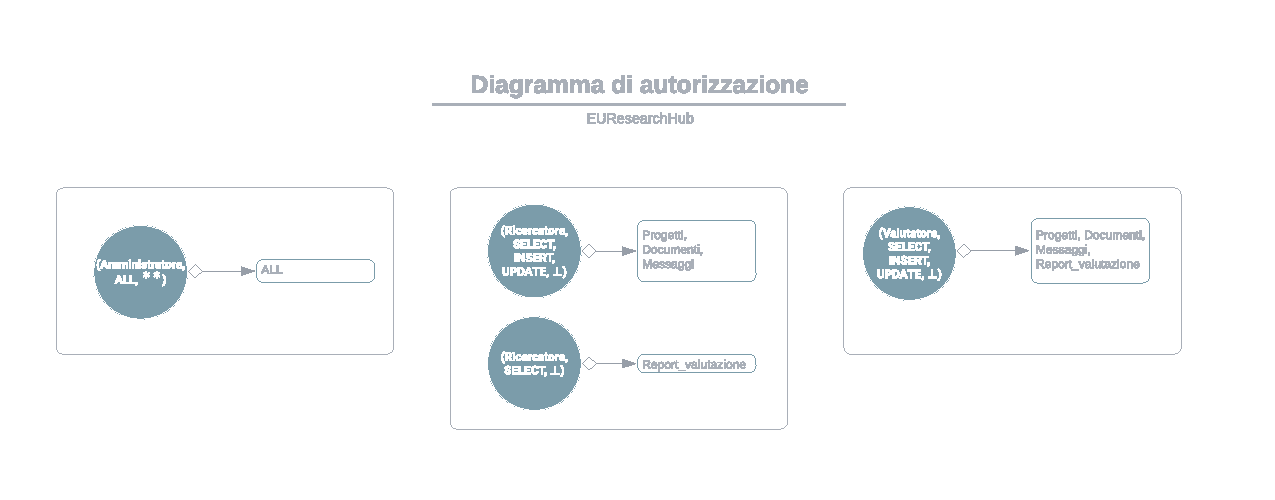
\includegraphics[scale = 0.7]{1.pdf}
\end{center}
Nel contesto descritto, non sembra necessario inserire ereditarietà o delega di permessi tra i ruoli, motivo per cui nel diagramma soprastante i nodi non sono legati tra di essi. Ogni ruolo ha responsabilità e permessi molto specifici e distinti, e non sembra esserci un caso d'uso in cui un ruolo avrebbe bisogno di ereditare i permessi di un altro ruolo.\\


\section{Progettazione concettuale}

Dopo l'analisi e raccolta dei requisiti il secondo pilastro necessario per la progettazione e modellazione del nostro database è la progettazione concettuale. Essa consente di strutturare gli elementi chiave del sistema prima identificati. Nel nostro caso, è stato utilizzato Lucidchart per sviluppare un modello ad oggetti che rappresenta le tabelle, le relazioni, i vincoli e le invarianti, fornendo una panoramica comprensiva e astratta dell'architettura del database.\\
Nel modello concettuale, le tabelle rappresentano le entità principali del sistema, come i ricercatori, i valuatori, i progetti, i documenti e così via. Le relazioni tra queste entità sono state modellate con parzialità e molteplicità, indicando come le diverse entità interagiscono tra loro e quali sono le dipendenze tra di esse.\\
Gli invarianti sono stati evidenziati infondo alle tabelle interessate per garantire l'integrità e la consistenza dei dati. Ad esempio, alcuni dei vincoli menzionati in precedenza, come il controllo sulla lunghezza delle password e il formato degli indirizzi email, sono stati inclusi nel modello per assicurare che i dati inseriti nel sistema rispettino le regole e standard.
\subsection{Schema ad oggetti}
\begin{sidewaysfigure}
\centering
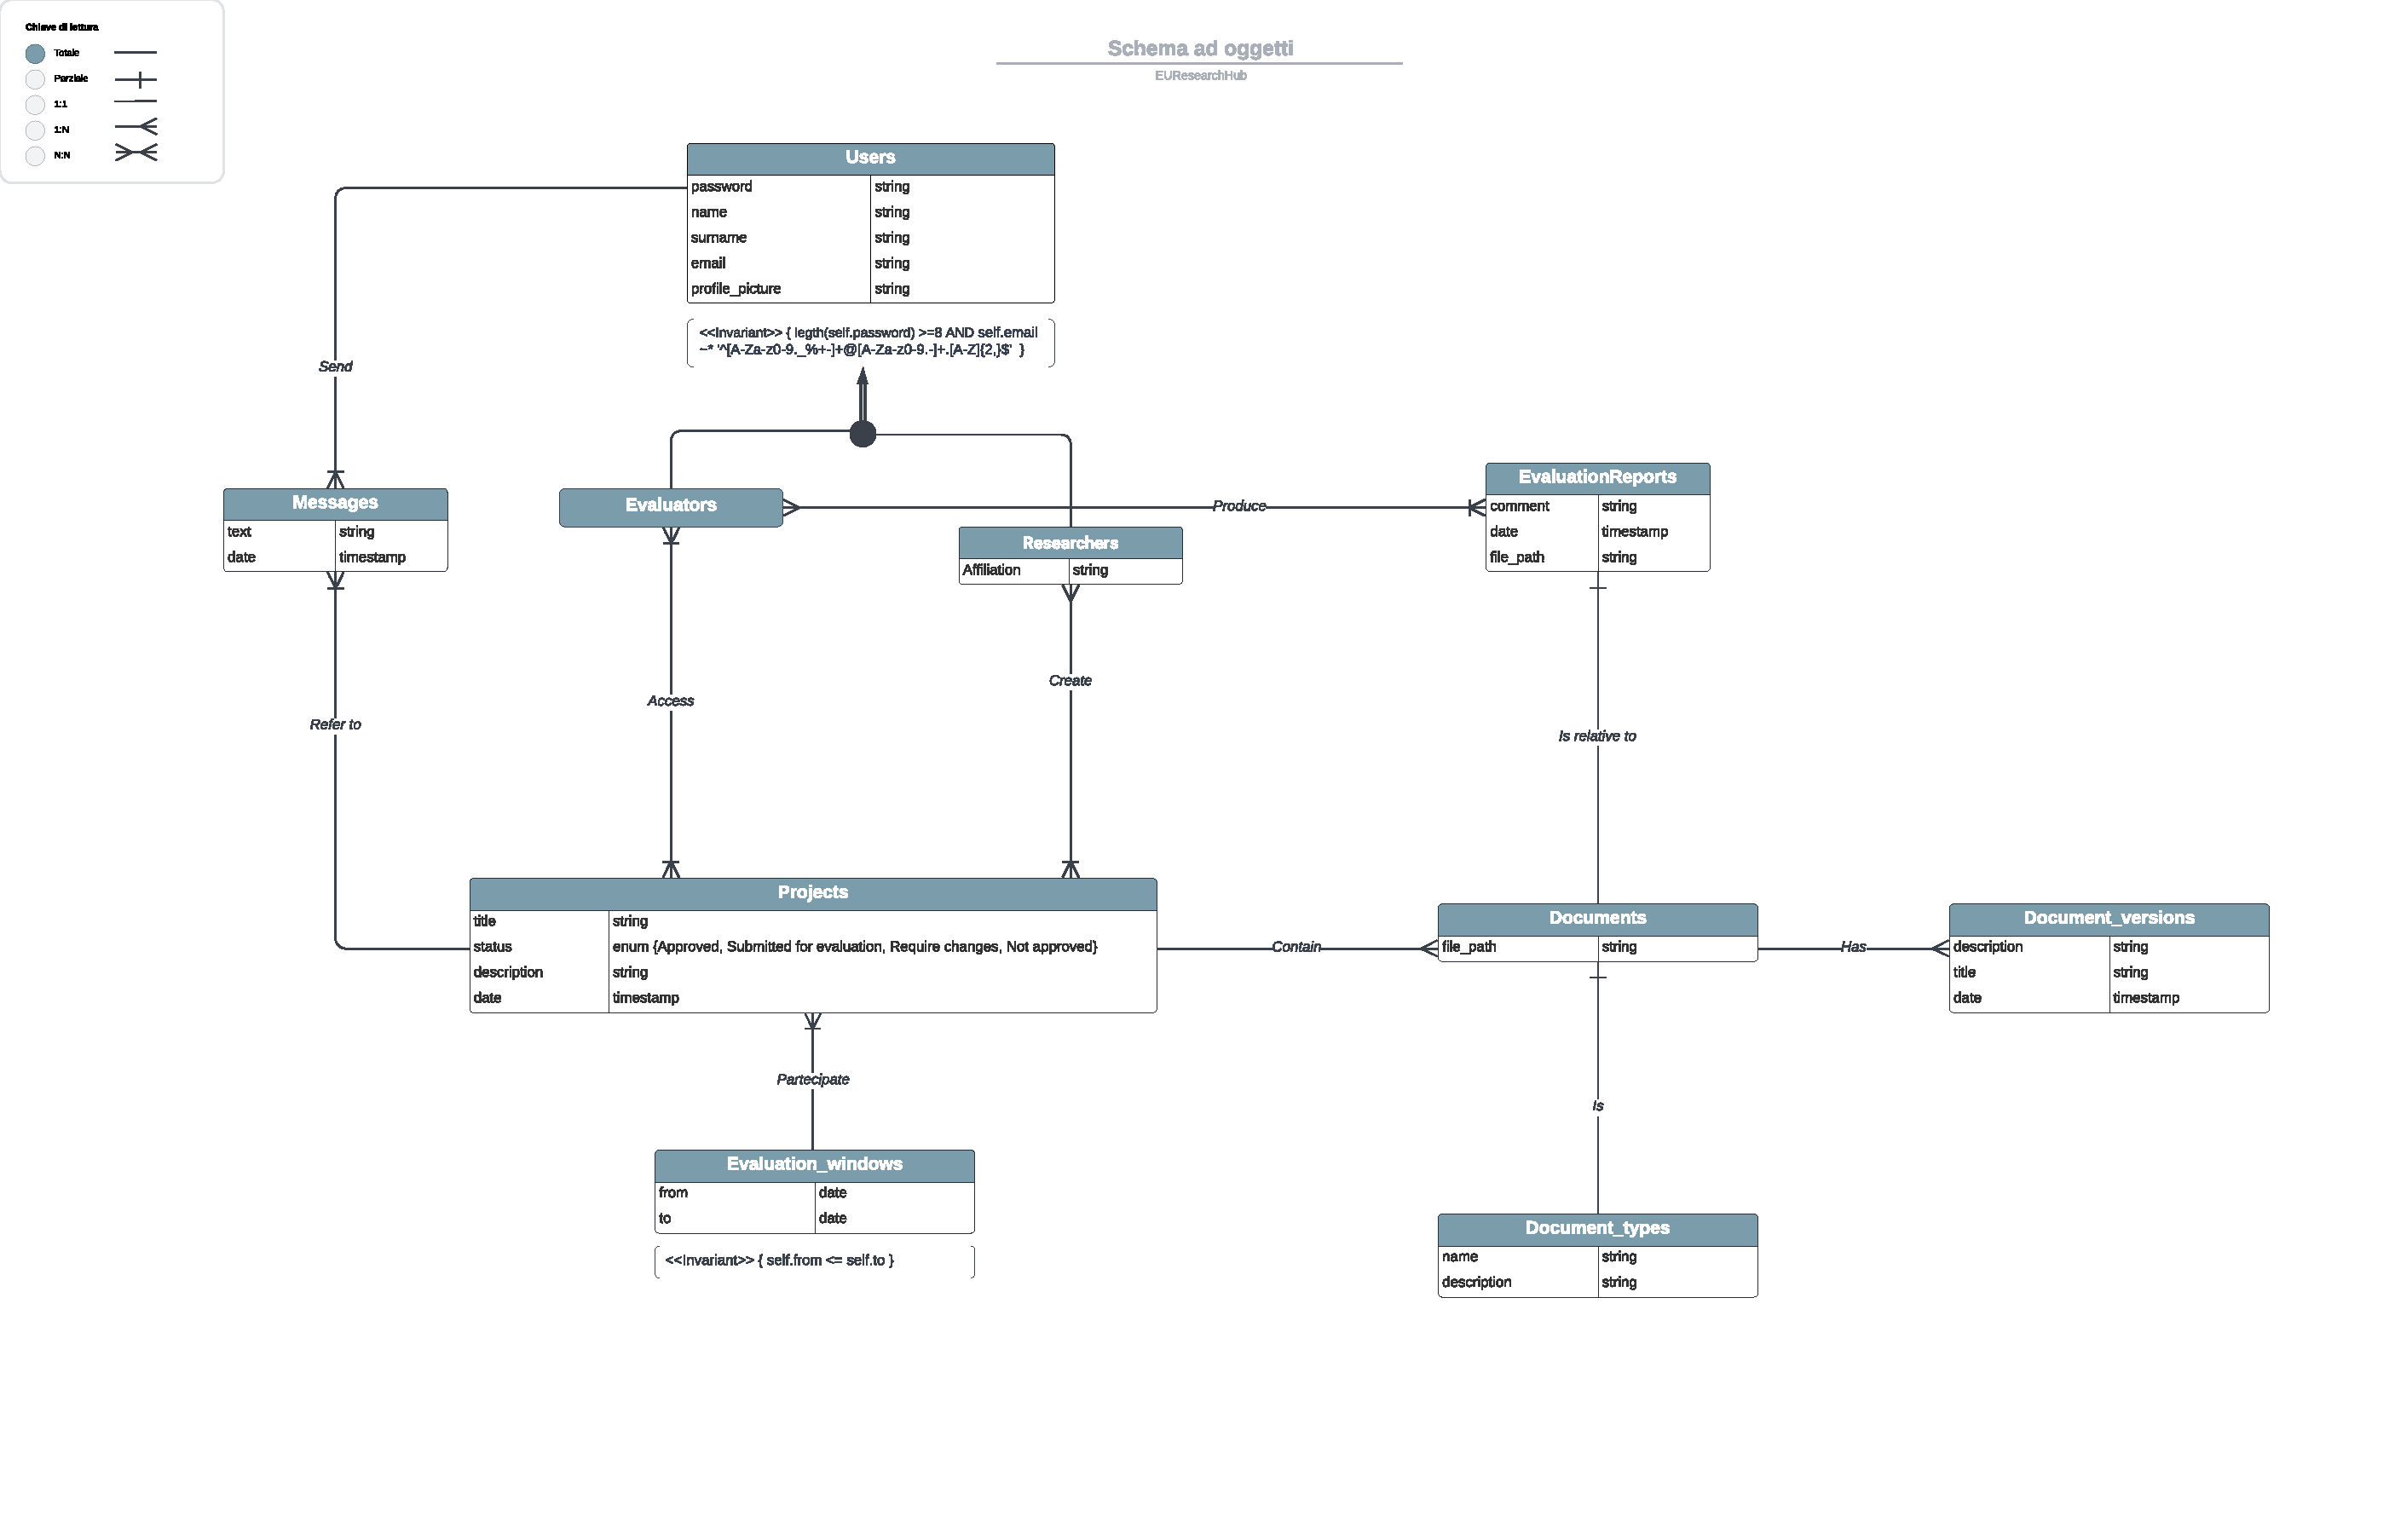
\includegraphics[width=1.00\textwidth]{Schema a oggetti.pdf}
\caption{Schema ad oggetti}
\end{sidewaysfigure}
\newpage
\subsection{Giustificazione delle decisioni progettuali}
Di seguito sono riportate le giustificazioni delle principali decisioni progettuali per garantire che il sistema fosse scalabile, efficiente e facile da mantenere:
\begin{itemize}
\item \textbf{Utilizzo di tipi enum:} Per rappresentare lo status dei progetti, creeremo un tipo enumerato \imtaInlinecode{latex}{enum_status}. Questo garantisce che solo i valori predefiniti possano essere inseriti nella colonna status della tabella \imtaInlinecode{latex}{projects}, garantendo la consistenza dei dati e facilitando le query sullo stato dei progetti.

\item \textbf{Definita una relazione di sottoclasse:} Sono state definite due sottoclassi partizione \imtaInlinecode{latex}{researchers} e \imtaInlinecode{latex}{evaluators} che ereditano gli attributi da \imtaInlinecode{latex}{users} per evitare eventuali ridondanze e permettere durante la progettazione logica di effettuare l'implementazione corretta.

\item \textbf{Suddivisione delle informazioni in tabelle separate:} Al fine di garantire la normalizzazione del database e ridurre la ridondanza dei dati, le informazioni sono state suddivise in tabelle separate. Ad esempio, le informazioni sui documenti e le loro versioni sono state divise nelle tabelle \imtaInlinecode{latex}{documents} e \imtaInlinecode{latex}{document_versions}, permettendo di gestire più versioni di uno stesso documento in modo efficiente. In maniera analoga anche le \imtaInlinecode{latex}{evaluation_windows} vengono salvate in una tabella separata da \imtaInlinecode{latex}{projects}.

\item \textbf{Utilizzo di invarianti:} già accennate in precedenza.

\end{itemize}


\section{Progettazione logica}
Ora analizziamo la fase intermedia della nostra modellazione: La progettazione logica. 
In questa fase, abbiamo tradotto il modello concettuale ad oggetti in uno schema logico che è stato utilizzato poi durante la creazione del database. La progettazione logica è essenziale per diverse ragioni:
\begin{enumerate}
\item Consente di identificare e risolvere eventuali problemi nella struttura dei dati prima di passare alla progettazione fisica.
\item Semplifica la mappatura tra il modello concettuale e il modello fisico, riducendo il rischio di errori e migliorando la coerenza dei dati.
\item Fornisce un'opportunità per ottimizzare le prestazioni del database, ad esempio selezionando gli indici appropriati e creando viste materializzate per migliorare l'efficienza delle query che si andranno ad implementare durante la progettazione fisica.
\end{enumerate}

\subsection{Schema logico}
\begin{sidewaysfigure}
\centering
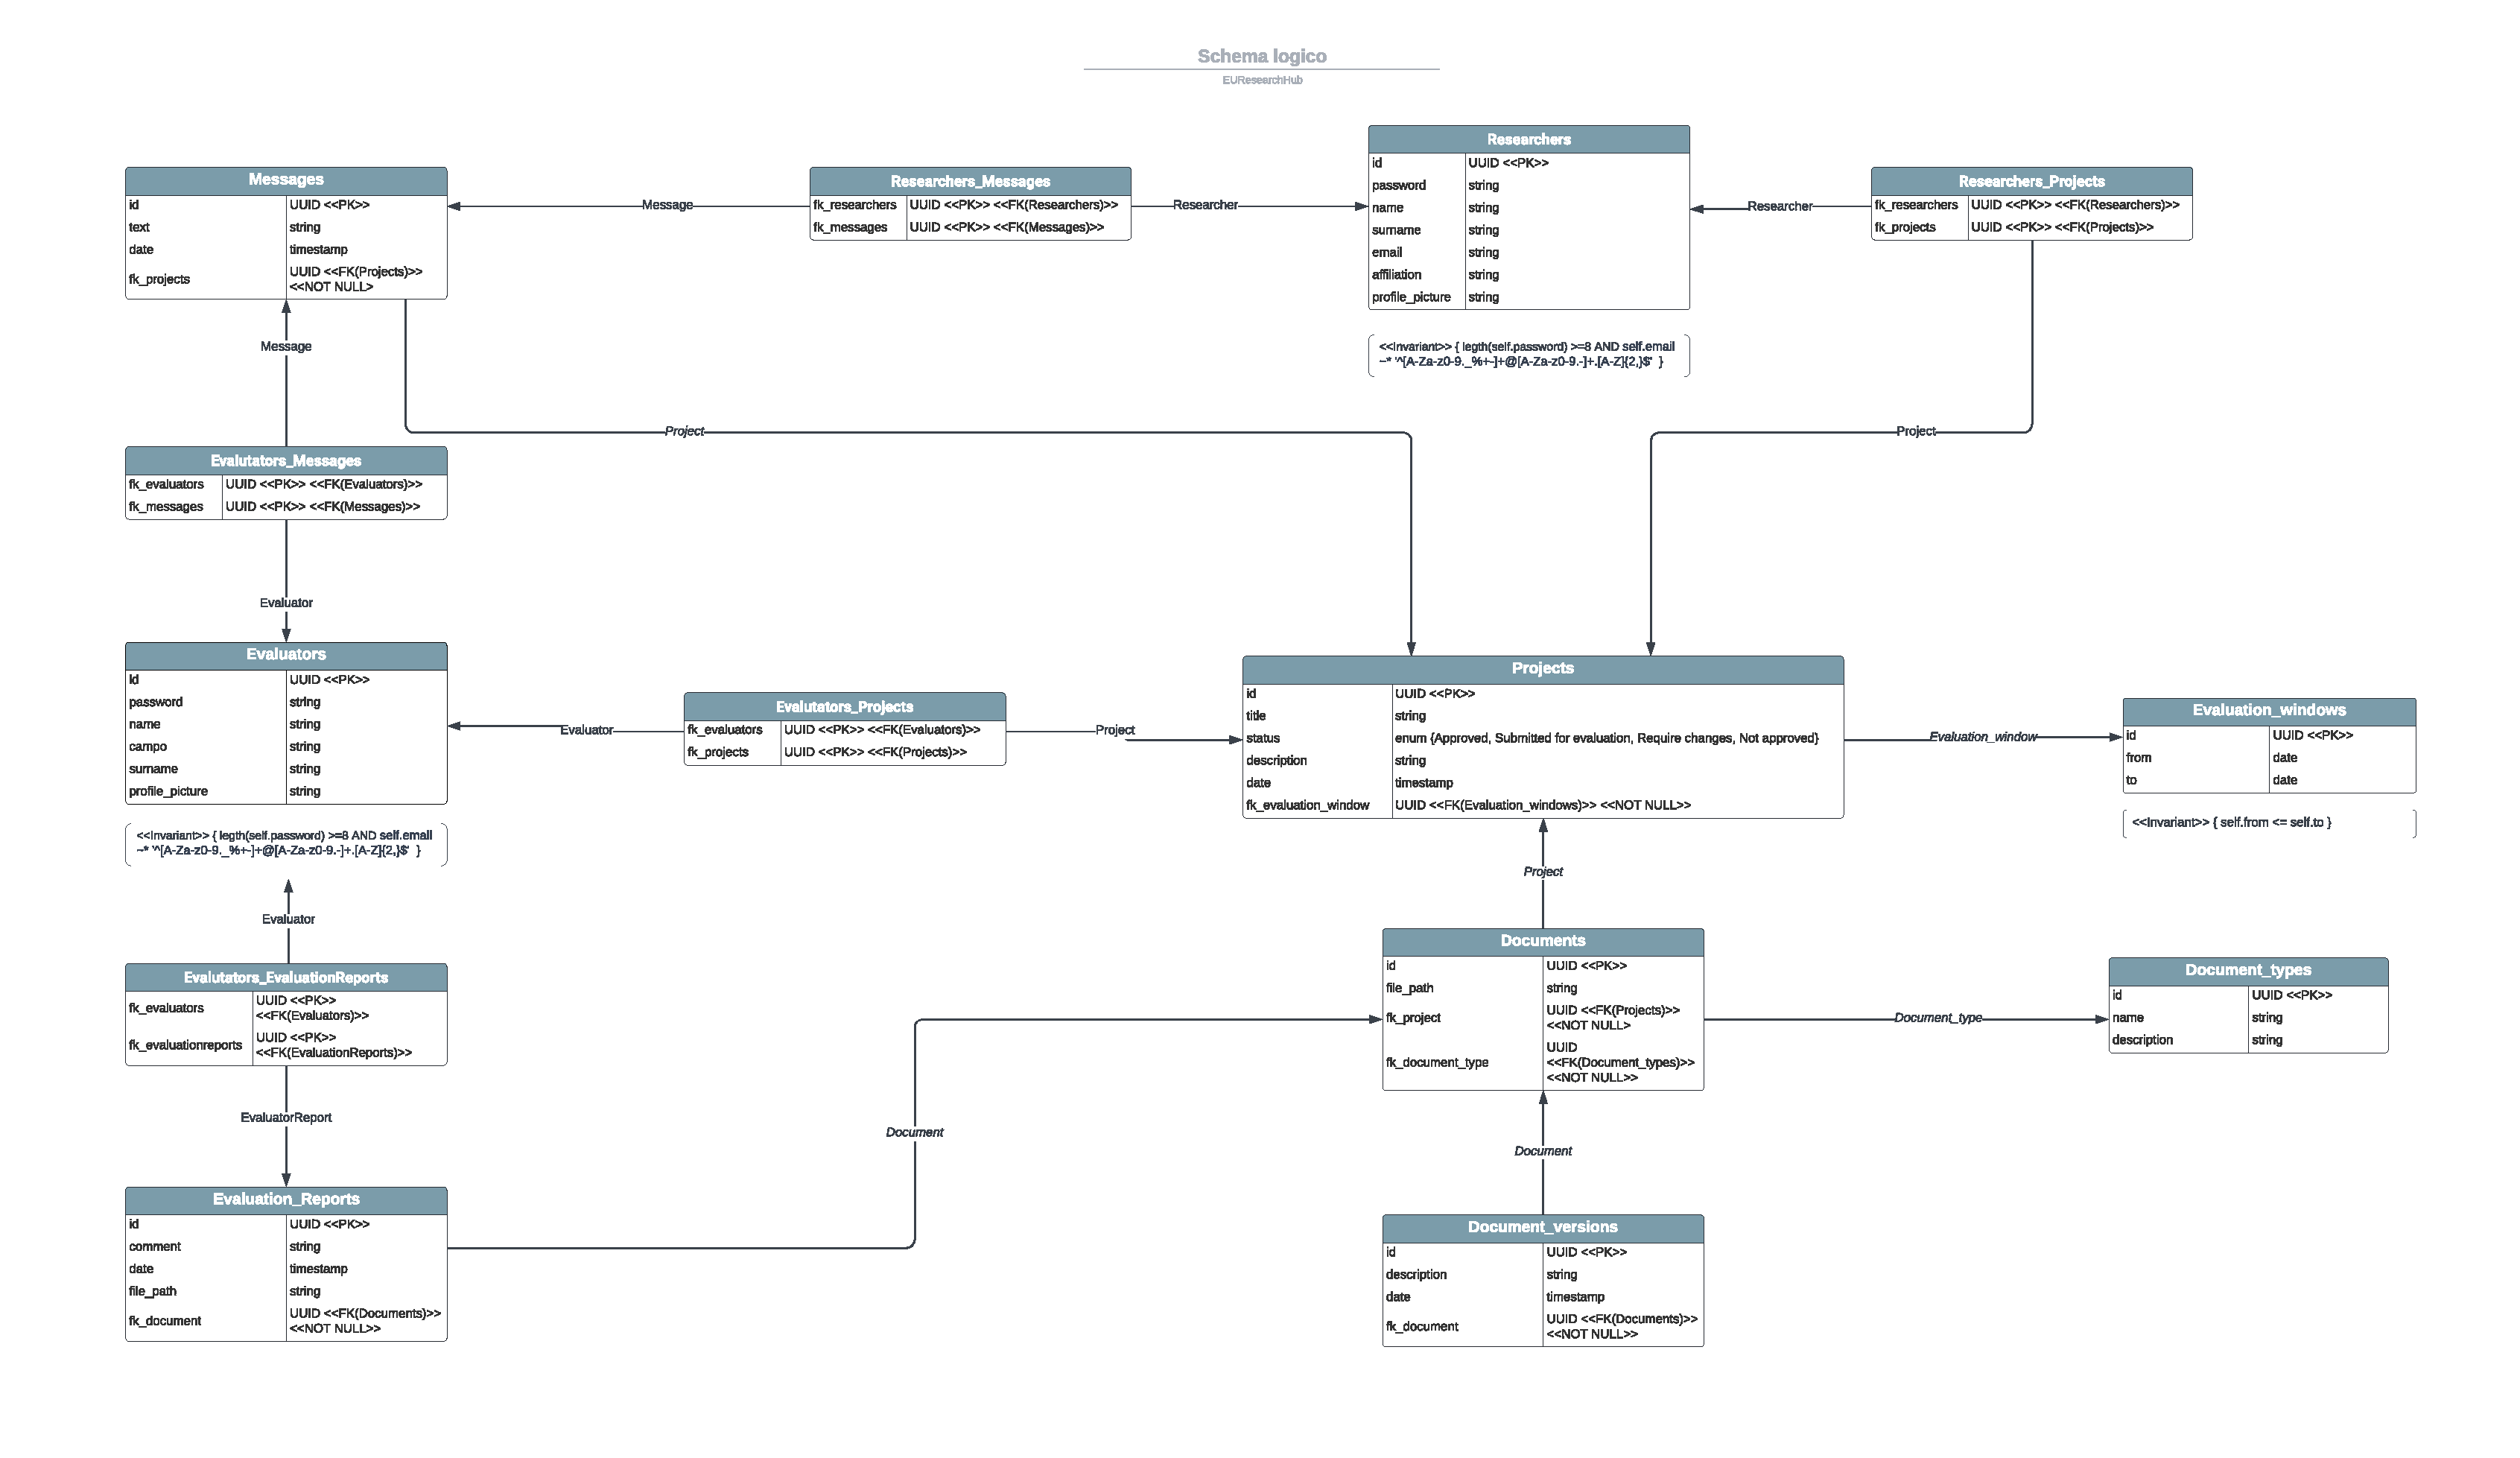
\includegraphics[width=1.00\textwidth]{Schema logico.pdf}
\caption{Schema logico}
\end{sidewaysfigure}
\newpage
\subsection{Giustificazione delle decisioni progettuali}
Di seguito sono riportate le giustificazioni di alcune delle decisioni chiave per questa fase:
\begin{itemize}

\item\textbf{ Tradotta la relazione di sottoclasse tramite partizionamento orizzontale:} Dalla gerarchia iniziale si è arrivati a suddividere le due sottoclassi partizione \imtaInlinecode{latex}{researchers} e \imtaInlinecode{latex}{evaluators}  in due tabelle a se stanti che ereditano gli attributi da \imtaInlinecode{latex}{users} poiché non si voleva complicare maggiormente la vista di tutti gli elementi della super classe tramite partizionamento verticale e neanche generalizzare troppo utilizzando una discriminante e ragruppando tutti gli attributi nella tabella unica \imtaInlinecode{latex}{users}.

\item \textbf{Chiavi esterne e relazioni:} Sono state utilizzate chiavi esterne per stabilire relazioni tra le diverse tabelle, garantendo l'integrità referenziale e semplificando le query tra tabelle correlate. Ad esempio, la tabella \imtaInlinecode{latex}{documents} ha una chiave esterna che fa riferimento alla tabella \imtaInlinecode{latex}{projects}, indicando a quale progetto appartiene ciascun documento.

\item \textbf{Utilizzo di tabelle intermedie per relazioni molti-a-molti:} Per gestire le relazioni molti-a-molti tra entità, sono state create tabelle intermedie, come \imtaInlinecode{latex}{researchers_projects} e \imtaInlinecode{latex}{evaluators_messages}. Queste tabelle consentono di associare più ricercatori a più progetti e più messaggi a più valutatori, garantendo la flessibilità del sistema e semplificando le query tra tabelle correlate.

\item \textbf{Inserito \imtaInlinecode{latex}{id} univoco per ogni tabella:} Ogni tabella è caratterizzata da un ID univoco sotto forma di intero auto incrementato.

\item \textbf{Inserito vincolo \imtaInlinecode{latex}{UNIQUE} sulle mail:} Ogni utente è caratterizzata da un email che deve essere univoco.


\end{itemize}


\section{Progettazione fisica}
La progettazione fisica presenta l'ultima stazione per completare questo capitolo.  Vista l'analisi a 360° del database, e di come dovrebbe funzionare l'applicativo non resta che applicare le osservazioni fatte su DBeaver. I costrutti per la creazione si basano sul linguaggio PostgreSQL.
\subsection{Istruzioni \texttt{SQL}}
Per le istruzioni SQL di creazione della base di dati si veda allegato \imtaInlinecode{latex}{dump.sql}. 

\subsection{Specifiche integrità dei dati}
Definite le tabelle in SQL chiave risulta fondamentale implementare i vincoli individuati durante la raccolta ed analisi dei requisiti e aggiungerne nuovi individuati durante la progettazione.  
Più in dettaglio, i vincoli definitivi implementati in PosgreSQL sono stati:\\
\phantom{This text will be invisible}\\
Vincolo sulla tabella \imtaInlinecode{latex}{evaluation_windows}
\begin{imtaCode}{PostgreSQL}
ALTER TABLE "EUResearchHub".evaluation_windows
ADD CONSTRAINT evaluation_windows_dates_check CHECK ("from" <= "to");
\end{imtaCode}
\phantom{This text will be invisible}\\
Vincoli sulla lunghezza delle password per le due tipologie di users \imtaInlinecode{latex}{researchers} ed \imtaInlinecode{latex}{evaluators}
\begin{imtaCode}{PostgreSQL}
ALTER TABLE "EUResearchHub".researchers
ADD CONSTRAINT researchers_password_length_check CHECK (LENGTH("password") >= 8);

ALTER TABLE "EUResearchHub".evaluators
ADD CONSTRAINT evaluators_password_length_check CHECK (LENGTH("password") >= 8);
\end{imtaCode}
\phantom{This text will be invisible}\\
Vincoli sull'email per \imtaInlinecode{latex}{researchers} ed \imtaInlinecode{latex}{evaluators}:
\begin{imtaCode}{PostgreSQL}
ALTER TABLE "EUResearchHub".researchers
ADD CONSTRAINT researchers_email_check CHECK (email ~* '^[A-Za-z0-9._%+-]+@[A-Za-z0-9.-]+\.[A-Z]{2,}$');

ALTER TABLE "EUResearchHub".evaluators
ADD CONSTRAINT researchers_email_check CHECK (email ~* '^[A-Za-z0-9._%+-]+@[A-Za-z0-9.-]+\.[A-Z]{2,}$');
\end{imtaCode}
L'utilità del vincolo è gia stata spiegata ma risulta interessante, in questo caso, spigarne i tecnicismi. Il vincolo utilizza una regex (espressione regolare). Per comprenderne meglio il funzionamento possiamo dividere la stringa in 4 parti: 

\begin{enumerate}
\item \textbf{\^[A-Za-z0-9.\_\%+-]+}: questa parte dell'espressione indica che l'indirizzo email deve iniziare (\^) con una sequenza di almeno un carattere (+) che può essere una lettera maiuscola o minuscola, un numero, un punto, un underscore, un simbolo di percentuale, un simbolo più o un simbolo meno.
\item \textbf{@}: questo simbolo indica che, dopo la sequenza iniziale di caratteri, deve essere presente il simbolo "@" che separa la parte locale dell'indirizzo email dal dominio.
\item \textbf{[A-Za-z0-9.-]+}: questa parte dell'espressione indica che, dopo il simbolo "@", deve esserci una sequenza di almeno un carattere (+) che può essere una lettera maiuscola o minuscola, un numero, un punto o un trattino. Questa sequenza rappresenta il dominio dell'indirizzo email (ad esempio, "gmail.com" o "example.org").
\item \textbf{ \.[A-Z]{2,}\$}: questa parte finale dell'espressione indica che, dopo il dominio, deve essere presente un punto seguito da almeno due lettere maiuscole o minuscole ({2,}). Questa sequenza rappresenta il suffisso del dominio, come ".com", ".org" o ".net". Il simbolo \$ alla fine dell'espressione indica che la stringa deve terminare con il suffisso del dominio.
\end{enumerate}

\phantom{This text will be invisible}\\
Trigger sulla tabella  \imtaInlinecode{latex}{document_versions}:
\begin{imtaCode}{PostgreSQL}
CREATE FUNCTION check_document_version_date()
RETURNS TRIGGER AS $$
DECLARE
  previous_version_date TIMESTAMP;
BEGIN
  SELECT "date" INTO previous_version_date
  FROM "EUResearchHub".document_versions
  WHERE fk_document = NEW.fk_document
  ORDER BY "date" DESC
  LIMIT 1;

  IF previous_version_date IS NOT NULL AND previous_version_date >= NEW."date" THEN
    RAISE EXCEPTION 'New document version date must be greater than the previous version date';
  END IF;

  RETURN NEW;
END;
$$ LANGUAGE plpgsql;

CREATE TRIGGER check_document_versions_date
  BEFORE INSERT ON "EUResearchHub".document_versions
  FOR EACH ROW
  EXECUTE FUNCTION check_document_version_date();
\end{imtaCode}
Il trigger \imtaInlinecode{latex}{check_document_versions_date} è stato creato per verificare che la data della nuova versione di un documento (NEW.date) sia sempre maggiore rispetto alla data dell'ultima versione registrata nella base di dati. La funzione \imtaInlinecode{latex}{check_document_version_date()} viene eseguita prima dell'inserimento di una nuova versione del documento nella tabella \imtaInlinecode{latex}{document_versions}. Se la condizione non è soddisfatta, viene generato un errore e l'operazione di inserimento viene interrotta. Questo trigger garantisce che le versioni dei documenti siano sempre ordinate in modo cronologico, facilitando la gestione delle modifiche e delle revisioni dei documenti.

\phantom{This text will be invisible}\\
Trigger sulla tabella  \imtaInlinecode{latex}{projects}:
\begin{imtaCode}{PostgreSQL}
CREATE FUNCTION check_project_status_change()
RETURNS TRIGGER AS $$
DECLARE
  document_count INTEGER;
  evaluated_document_count INTEGER;
BEGIN
  SELECT COUNT(*) INTO document_count
  FROM "EUResearchHub".documents
  WHERE fk_project = NEW.id;

  SELECT COUNT(DISTINCT d.id) INTO evaluated_document_count
  FROM "EUResearchHub".documents d
  JOIN "EUResearchHub".evaluation_reports er ON d.id = er.fk_document
  WHERE d.fk_project = NEW.id;

  IF document_count <> evaluated_document_count THEN
    RAISE EXCEPTION 'Cannot change the status of a project if not all documents have been evaluated';
  END IF;

  RETURN NEW;
END;
$$ LANGUAGE plpgsql;

CREATE TRIGGER check_projects_status_change
  BEFORE UPDATE ON "EUResearchHub".projects
  FOR EACH ROW
  WHEN (OLD.status <> NEW.status AND NEW.status IN ('approved', 'require changes', 'not approved'))
  EXECUTE FUNCTION check_project_status_change();
\end{imtaCode}
Il trigger \imtaInlinecode{latex}{check_projects_status_change} è stato sviluppato per garantire che lo stato di un progetto possa essere modificato solo se tutti i documenti associati al progetto sono stati valutati. La funzione associata viene eseguita prima dell'aggiornamento dello stato del progetto nella tabella \imtaInlinecode{latex}{projects}. Se la condizione non è soddisfatta, viene generato un errore e l'operazione di aggiornamento viene interrotta. Questo trigger assicura che i progetti non vengano approvati, richiedano modifiche o siano respinti finché non vengono completamente valutati, garantendo un processo di valutazione accurato e completo.\\
\phantom{This text will be invisible}\\
Trigger sulle tabelle  \imtaInlinecode{latex}{researchers} e \imtaInlinecode{latex}{evaluators}:
\begin{imtaCode}{PostgreSQL}
CREATE FUNCTION check_unique_email()
  RETURNS TRIGGER AS
$$
BEGIN
  IF EXISTS (SELECT 1 FROM "EUResearchHub".researchers WHERE email = NEW.email) THEN
    RAISE EXCEPTION 'Another user is usinng this email, please change it';
  END IF;

  IF EXISTS (SELECT 1 FROM "EUResearchHub".evaluators WHERE email = NEW.email AND id <> NEW.id) THEN
    RAISE EXCEPTION 'Another user is usinng this email, please change it';
  END IF;

  RETURN NEW;
END;
$$
LANGUAGE plpgsql;

CREATE TRIGGER check_unique_email_insert_update
BEFORE INSERT OR UPDATE ON "EUResearchHub".evaluators
FOR EACH ROW
EXECUTE FUNCTION check_unique_email();
CREATE TRIGGER check_unique_email_insert_update
BEFORE INSERT OR UPDATE ON "EUResearchHub".researchers
FOR EACH ROW
EXECUTE FUNCTION check_unique_email();
\end{imtaCode}
Il trigger \imtaInlinecode{latex}{check_unique_email} viene utilizzato per garantire che le email siano uniche tra le tabelle \imtaInlinecode{latex}{researchers} e \imtaInlinecode{latex}{evaluators}. Ciò significa che un ricercatore non può essere anche un valutatore, in quanto il loro indirizzo email deve essere univoco in entrambe le tabelle.  Questo trigger, oltre a permettere di far rispettare la scelta della tipologia gerarchica di \imtaInlinecode{latex}{users} presa durante la progettazione concettuale risulta utile anche perché l'immagine del profilo durante lo sviluppo verrà salvata salvate come \imtaInlinecode{latex}{email.pdf}. La funzione associata al trigger esegue i seguenti controlli:
\begin{itemize}
\item Verifica se l'email inserita esiste già nella tabella \imtaInlinecode{latex}{researchers}. Se l'email viene trovata, viene generata un'eccezione con un messaggio di errore appropriato. Questo assicura che un ricercatore non possa essere inserito come valutatore se la sua email è già presente nella tabella \imtaInlinecode{latex}{researchers}.
\item Verifica se l'email inserita esiste già nella tabella \imtaInlinecode{latex}{evaluators}, escludendo la riga corrente dall'operazione di controllo. Questo è necessario per consentire l'aggiornamento di altre colonne nella tabella \imtaInlinecode{latex}{evaluators} senza generare un'eccezione di duplicazione email. Ad esempio, se un valutatore cambia il suo nome o cognome, l'aggiornamento dovrebbe essere consentito anche se l'email esiste già. \item Tuttavia, se l'email viene trovata su una riga diversa da quella corrente, viene generata un'eccezione per evitare la duplicazione dell'email tra i valutatori.
\item Se nessuna corrispondenza viene trovata in entrambe le tabelle, l'email è considerata unica e il trigger restituisce la nuova riga per l'inserimento o l'aggiornamento.
\end{itemize}


\subsection{Gestione dei ruoli e politiche di autorizzazione}
Un altro step, già iniziato durante la raccolta ed analisi dei requisiti e che finalmente possiamo implementare è la gestione dei ruoli e delle politiche di autorizzazione. Come già accennato nel caso di EUResearchHub, sono stati definiti tre ruoli: \textbf{Admin}, \textbf{Researcher} e \textbf{Evaluator}. \\
Nello specifico i tre ruoli sono stati implementati come segue:\\
L'utente \textbf{Admin} ha privilegi di superutente, il che significa che può accedere a tutte le tabelle e eseguire qualsiasi operazione sullo schema EUResearchHub. Questo ruolo è utile per la gestione e la manutenzione del sistema e sarà  limitato a un ristretto numero di utenti (ipoteticamente utenti incaricati e dipendenti dell'unione europea che si occupano di mantenere il servizio).
\begin{imtaCode}{PostgreSQL}
CREATE ROLE "Admin" SUPERUSER CREATEDB CREATEROLE NOINHERIT LOGIN NOREPLICATION BYPASSRLS PASSWORD '****';
GRANT ALL PRIVILEGES ON SCHEMA "EUResearchHub" TO "Admin";
\end{imtaCode}
Il ruolo del \textbf{Researcher} consente l'accesso alle tabelle relative ai documenti, ai tipi di documento, ai progetti, ai messaggi e alle associazioni tra ricercatori e progetti. I ricercatori possono inserire e modificare le informazioni relative ai loro progetti e documenti, ma non possono accedere alle tabelle degli evaluatori.
\begin{imtaCode}{PostgreSQL}
CREATE ROLE Researcher NOSUPERUSER NOCREATEDB NOCREATEROLE NOINHERIT LOGIN NOREPLICATION NOBYPASSRLS PASSWORD '****';
GRANT SELECT ON TABLE "EUResearchHub".document_types TO researcher;
GRANT INSERT, SELECT ON TABLE "EUResearchHub".document_versions TO researcher;
GRANT INSERT, DELETE, SELECT ON TABLE "EUResearchHub".documents TO researcher;
GRANT SELECT ON TABLE "EUResearchHub".evaluation_reports TO researcher;
GRANT SELECT ON TABLE "EUResearchHub".evaluation_windows TO researcher;
GRANT INSERT, SELECT ON TABLE "EUResearchHub".messages TO researcher;
GRANT INSERT, DELETE, SELECT ON TABLE "EUResearchHub".projects TO researcher;
GRANT INSERT, SELECT ON TABLE "EUResearchHub".researchers_projects TO researcher;
GRANT SELECT ON TABLE "EUResearchHub".researchers_messages TO researcher;
\end{imtaCode}
Il ruolo dell'\textbf{Evaluator} permette di accedere alle tabelle relative ai documenti, ai tipi di documento, alle valutazioni e alle finestre di valutazione. Gli evaluatori possono inserire report di valutazione, aggiungere commenti  ai documenti inserendo una nuova versione del documento e aggiornare lo stato dei progetti, ma non possono modificare direttamente i documenti o i progetti stessi.
\begin{imtaCode}{PostgreSQL}
CREATE ROLE Evaluator NOSUPERUSER NOCREATEDB NOCREATEROLE NOINHERIT LOGIN NOREPLICATION NOBYPASSRLS PASSWORD '4321';
GRANT SELECT ON TABLE "EUResearchHub".document_types TO evaluator;
GRANT SELECT,INSERT ON TABLE "EUResearchHub".document_versions TO evaluator;
GRANT SELECT ON TABLE "EUResearchHub".documents TO evaluator;
GRANT INSERT, SELECT ON TABLE "EUResearchHub".evaluation_reports TO evaluator;
GRANT SELECT ON TABLE "EUResearchHub".evaluation_windows TO evaluator;
GRANT INSERT ON TABLE "EUResearchHub".messages TO evaluator;
GRANT UPDATE, SELECT ON TABLE "EUResearchHub".projects TO evaluator;
GRANT SELECT ON TABLE "EUResearchHub".researchers TO evaluator;
GRANT SELECT ON TABLE "EUResearchHub".researchers_messages TO evaluator;
GRANT SELECT ON TABLE "EUResearchHub".researchers_projects TO evaluator;
\end{imtaCode}
Per quanto utilizzare ruoli permetta di evitare inconsistenze, ci sono anche alcune problematiche che possono sorgere se analizzato attentamente il problema. 
Le politiche di autorizzazione, consentono di imporre ulteriori ma necessarie restrizioni sull'accesso ai dati, e risolvere i problemi accennati. In particolare attraverso l'uso di \textbf{Row Level Security (RLS)}. RLS si può limitare l'accesso alle righe di una tabella in base a una condizione specificata nella politica.\\
Nel nostro caso, abbiamo forzato la Row Level Security sulla tabella \imtaInlinecode{latex}{projects} e creato la politica researcher\_project\_access\_policy. Questa politica limita l'accesso alle righe della tabella \imtaInlinecode{latex}{projects} ai soli ricercatori associati a un determinato progetto. In questo modo, i ricercatori possono vedere e modificare solo i progetti a cui sono associati, garantendo una maggiore sicurezza e protezione dei dati.
\begin{imtaCode}{PostgreSQL}
ALTER TABLE "EUResearchHub".projects FORCE ROW LEVEL SECURITY;
CREATE POLICY researcher_project_access_policy
  ON "EUResearchHub".projects
  USING (id IN (SELECT fk_projects FROM "EUResearchHub".researchers_projects WHERE fk_researchers = current_setting('eu_research_hub.current_user_id')::integer));
ALTER TABLE "EUResearchHub".projects FORCE ROW LEVEL SECURITY;
\end{imtaCode}

\subsection{Performance: indici e  materialized view }
Anche la performance del database è un aspetto cruciale durante la progettazione fisica, poiché può influenzare direttamente l'esperienza utente e le prestazioni generali del sistema. Per ottimizzare le prestazioni del database, si possono utilizzare indici, materialized view e procedure. Di seguito viene analizzata l'implementazione degli indici e delle materialized view individuate ed implementate in EUResearchHub soffermandoci non solo sui vantaggi ma anche sui svantaggi che consapevolpente, abbiamo tenuto in considerazione.  Questa scelta risulta in realtà momentanea; solo a webapp ultimata, si potrà effettivamente implementare la soluzione ideale definitiva tramite uno studio approfondito sulla distribuzione dei dati e log delle query ( \imtaInlinecode{latex}{ANALYZE} e \imtaInlinecode{latex}{EXPLAIN}). 
Ad ogni modo si suppone che utilizzando le seguenti implementazioni si abbia un aumento della performance:
\begin{itemize}
\item \imtaInlinecode{latex}{projects_status_idx}: questo indice viene creato sulla colonna status della tabella \imtaInlinecode{latex}{projects}. Gli indici su colonne frequentemente utilizzate nelle clausole WHERE delle query possono velocizzare notevolmente le operazioni di ricerca. I vantaggi di questo indice includono un accesso più rapido ai dati per le query che filtrano i progetti in base allo stato (utile per i valutatori) e un miglioramento delle prestazioni delle query complesse che coinvolgono la tabella \imtaInlinecode{latex}{projects}. Gli svantaggi includono un maggiore utilizzo dello spazio su disco e un potenziale rallentamento delle operazioni di inserimento, aggiornamento e cancellazione, poiché l'indice deve essere mantenuto coerente con i dati nella tabella. Ipotizzando però che queste tipologie di operazioni avvengono raramente o in momenti specifici (i.e. inizio/fine di una finestra di valutazione) si è deciso ad ogni modo di implementare questo indice per ottimizzare l'user experience nel resto del tempo.\\

\begin{minipage}{\linewidth}
\begin{imtaCode}{PostgreSQL}
CREATE INDEX projects_status_idx ON "EUResearchHub".projects (status);
\end{imtaCode}
\end{minipage}


\item \imtaInlinecode{latex}{messages_fk_projects_idx}: questo indice viene creato sulla colonna fk\_projects della tabella \imtaInlinecode{latex}{messages}. Similmente all'indice precedente, l'obiettivo è di velocizzare le query che filtrano i messaggi in base al progetto associato. I vantaggi e gli svantaggi così come le scelte implementative sono simili a quelli dell'indice \imtaInlinecode{latex}{projects_status_idx}. Attraverso questa scelta progettuale vogliamo privilegiare la visualizzazione dei messaggi più che l'inserimento essendo comunque non una normale chat sottoposta continuamente a inserimento di messaggi (i.e. WhatsApp) ma utilizzata più raramente. \\

\begin{minipage}{\linewidth}
\begin{imtaCode}{PostgreSQL}
CREATE INDEX messages_fk_projects_idx ON "EUResearchHub".messages (fk_projects);
\end{imtaCode}
\end{minipage}


\item \imtaInlinecode{latex}{projects_status_count}: questa materialized view memorizza il conteggio dei progetti raggruppati per stato individuati utili nella pagina relativi a tutti i progetti. \\

\begin{minipage}{\linewidth}
\begin{imtaCode}{PostgreSQL}
CREATE MATERIALIZED VIEW projects_status_count AS
SELECT status, COUNT(*) as count
FROM "EUResearchHub".projects
GROUP BY status;
\end{imtaCode}
\end{minipage}

Per chiarezza si faccia riferimento alla seguente immagine:
\begin{center}
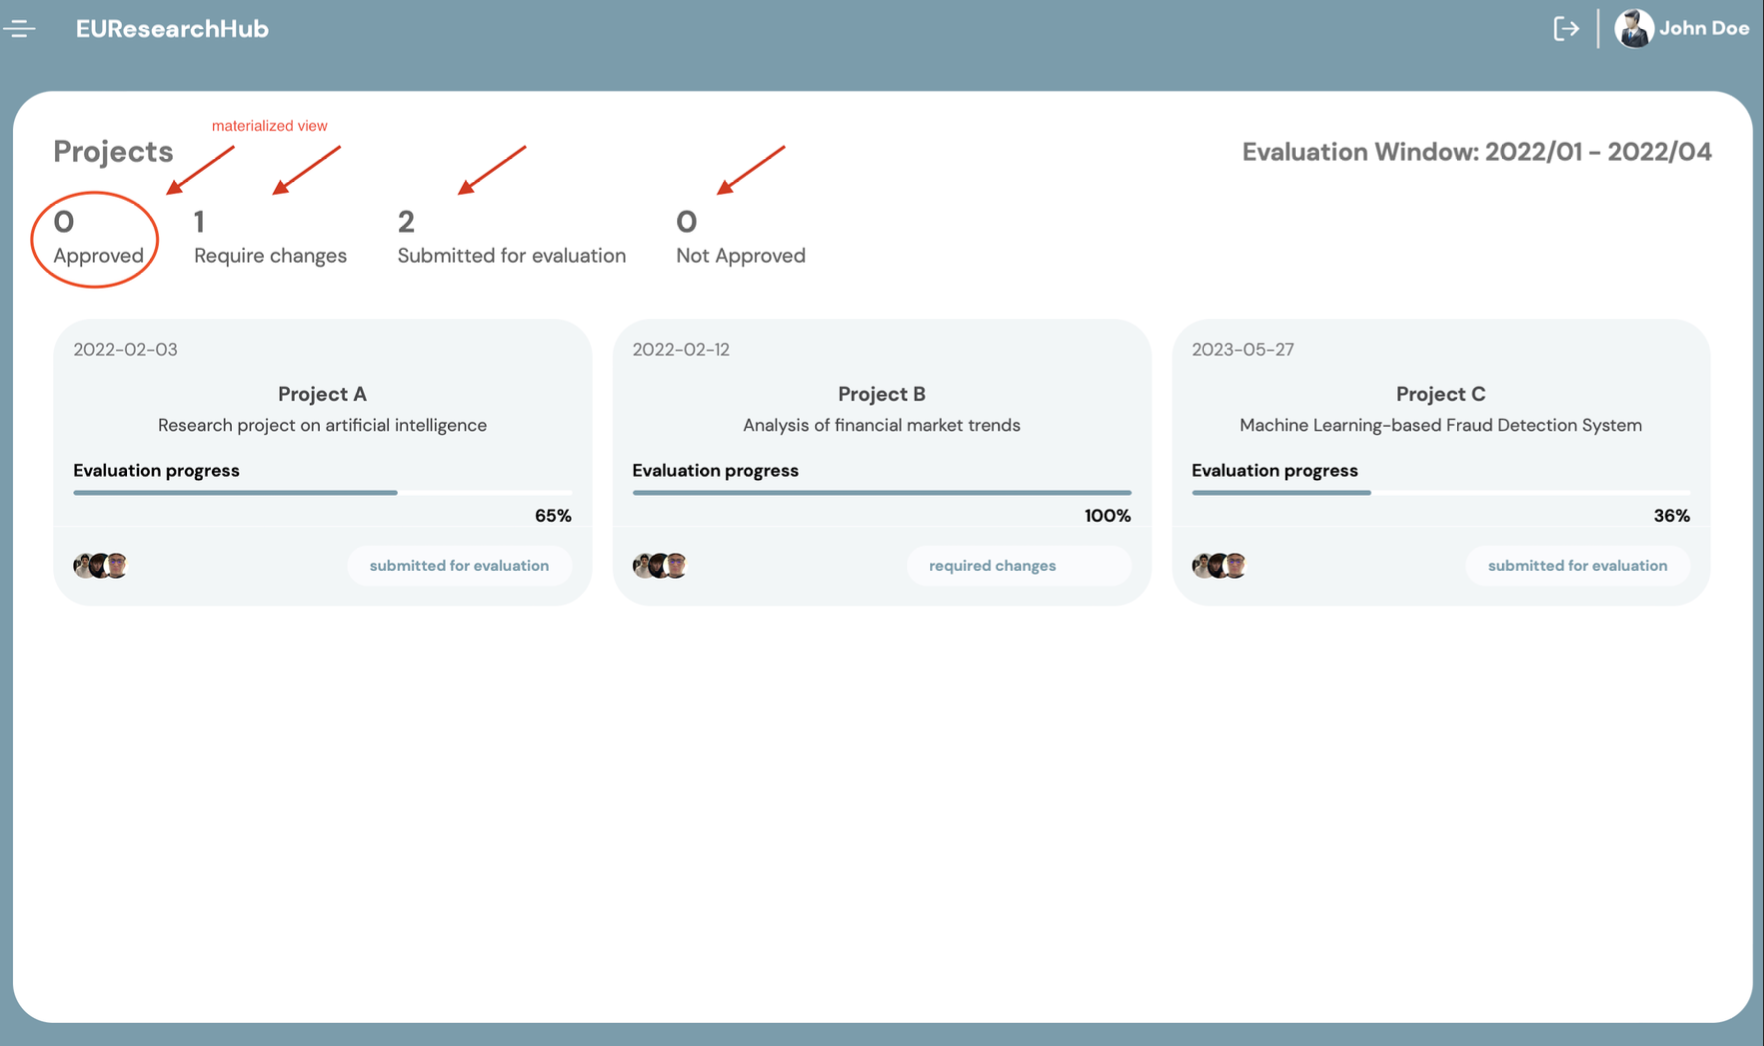
\includegraphics[scale = 0.04]{4.png}
\end{center}
I vantaggi di questa includono un accesso rapido al conteggio dei progetti per stato e un miglioramento delle prestazioni per le query che richiedono queste informazioni come nel caso sopra illustrato. Gli svantaggi includono un maggiore utilizzo dello spazio su disco e la necessità di aggiornare la materialized view ogni volta che i dati nella tabella \imtaInlinecode{latex}{projects} cambiano: indicamente alla fine di ogni finestra di valutazione.  Per fare fronte a questo ultimo problema abbiamo individuato due soluzioni: aggiornare la materialized view al termine di un evaluation window o a seguito di ogni aggiornamento che la potrebbe influenzare. Abbiamo deciso di optare per la seconda opzione e quindi abbiamo inserito un nuovo trigger \imtaInlinecode{latex}{refresh_project_status_count}, attivato solo a seguito di aggiornamento o inserimento di un nuovo status per ogni statement.  \\

\begin{minipage}{\linewidth}
\begin{imtaCode}{PostgreSQL}
CREATE FUNCTION "EUResearchHub".refresh_project_status_count()
 RETURNS trigger
 LANGUAGE plpgsql
AS $function$
BEGIN
  REFRESH MATERIALIZED VIEW projects_status_count;
  RETURN NEW;
END;
$function$
CREATE TRIGGER refresh_project_status_count_insert 
AFTER INSERT OR UPDATE
ON "EUResearchHub".projects 
FOR EACH STATEMENT
EXECUTE FUNCTION refresh_project_status_count()
\end{imtaCode}
\end{minipage}



\end{itemize}








.
\chapter{Sviluppo back-end}

\section{Scelta di Flask come framework}
Nella fase di progettazione del back-end di EUResearchHu,  abbiamo preso in considerazione diversi framework per lo sviluppo dell'applicazione web. Dopo un'attenta valutazione, abbiamo scelto Flask come framework principale per diverse ragioni.
Flask è un micro-framework leggero e flessibile scritto in Python che fornisce un set di strumenti essenziali per lo sviluppo di applicazioni web. 
Inoltre, Flask offre una vasta gamma di estensioni che consentono di estendere le funzionalità di base del framework per adattarsi alle esigenze specifiche del nostro progetto. Ad esempio, abbiamo utilizzato Flask-WTF per gestire i moduli e i token CSRF, semplificando la gestione della sicurezza dei form e delle richieste.
\section{Architettura dell'applicazione}
Per comprendere appieno il ruolo del back-end nel contesto dell'applicazione complessiva, è fondamentale analizzare l'architettura dell'applicazione nel suo insieme.
L'applicazione segue un'architettura a tre livelli, composta da front-end, back-end e database. \\
\subsection{Ruolo del back-end nell'architettura complessiva}
Il back-end svolge un ruolo centrale nel coordinare le richieste provenienti dal front-end e l'interazione con il database. Nel nostro caso riceve le richieste HTTP provenienti dal front-end e le elabora in modo appropriato. Ciò include l'elaborazione dei parametri delle richieste, la validazione dei dati in ingresso e il reindirizzamento delle richieste verso le funzioni di gestione corrispondenti.\\
\subsection{Organizzazione delle directory e dei file del progetto}
Il  sistema è organizzato in una struttura di directory ben definita, che favorisce una suddivisione logica dei file e delle risorse. Di seguito è riportato il dettaglio dell'albero delle directory principali:
\begin{center}
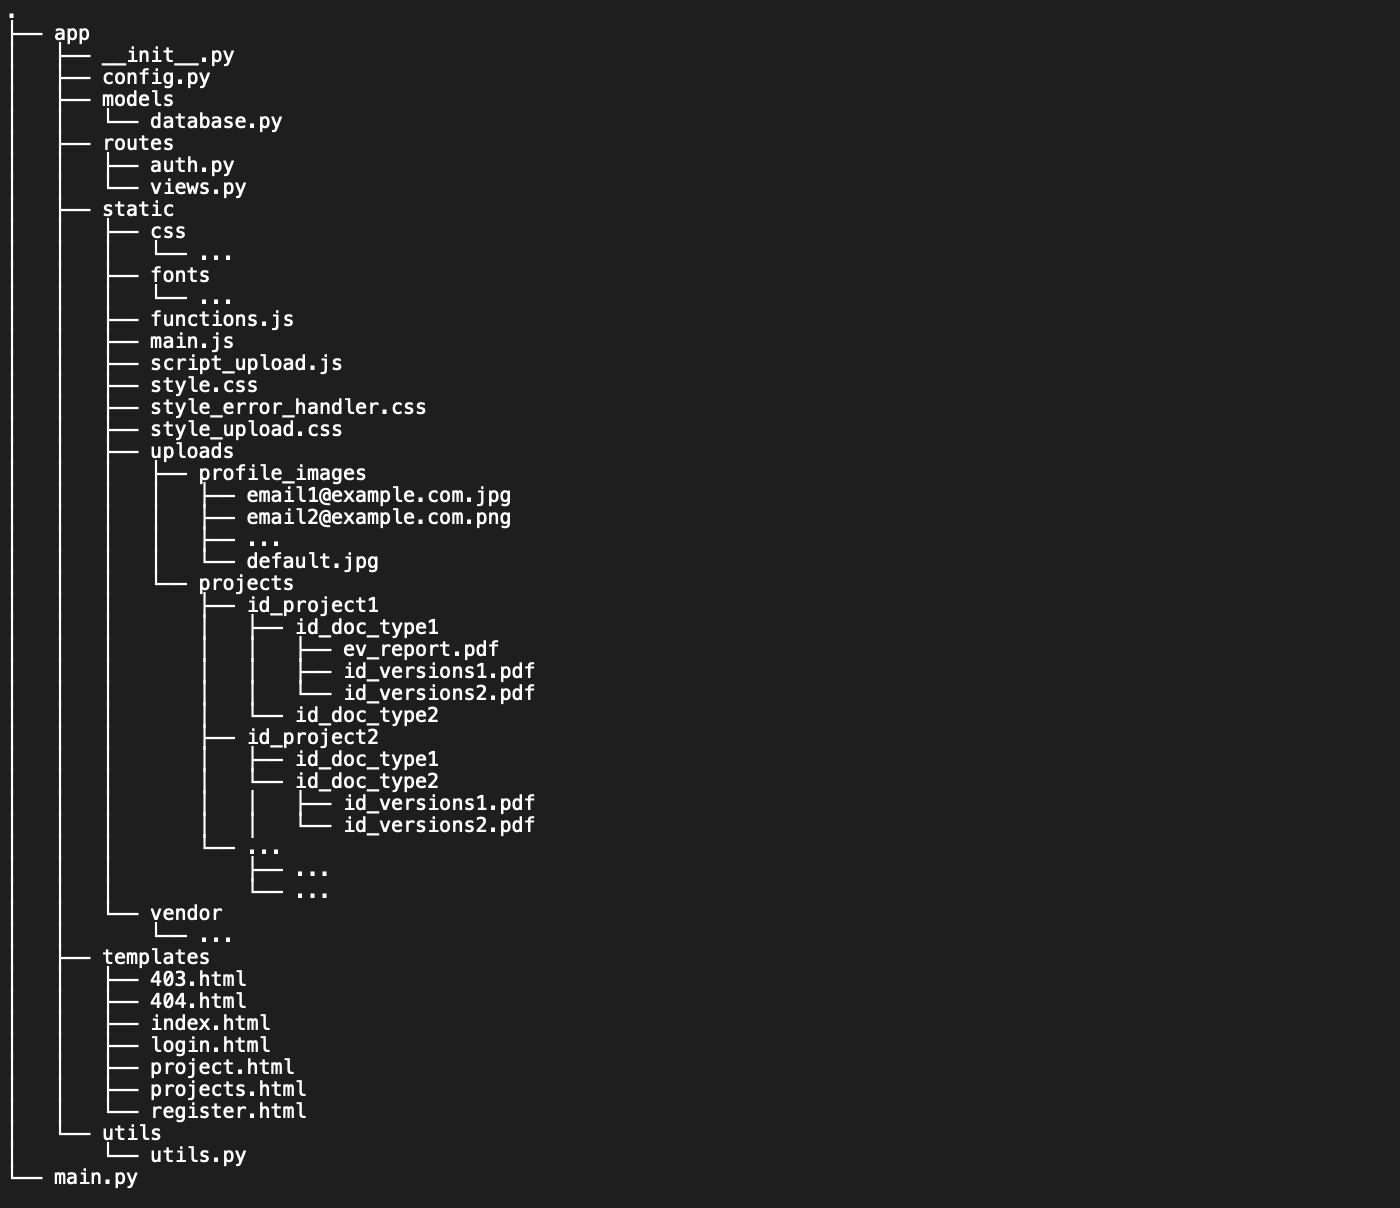
\includegraphics[scale = 0.5]{5.png}
\end{center}
\subsection{Principali componenti del back-end}
Come possiamo notare back-end del nostro progetto è costituito da diversi moduli e file di configurazione che lavorano in sinergia per fornire le funzionalità richieste. Ecco una panoramica delle principali componenti del back-end elencante della figura soprastante:
\begin{itemize}
\item \imtaInlinecode{latex}{init.py}: Questo file è il punto di ingresso dell'applicazione Flask. Viene utilizzato per inizializzare l'applicazione e configurarla prima dell'avvio del server.

\item \imtaInlinecode{latex}{config.py}: Questo file contiene la configurazione dell'applicazione, come la chiave segreta per la gestione delle sessioni, le impostazioni del database e altre variabili di configurazione.

\item \imtaInlinecode{latex}{models/database.py}: Questo modulo definisce le classi di modello che rappresentano le tabelle del database. Utilizziamo SQLAlchemy per semplificare l'interazione con il database PostgreSQL.

\item \imtaInlinecode{latex}{routes/auth.py}: Questo modulo contiene le route e le funzioni associate per la gestione dell'autenticazione e dell'autorizzazione degli utenti, come il login, la registrazione e il logout.

\item \imtaInlinecode{latex}{routes/views.py}: Questo modulo contiene le route e le funzioni associate per la gestione delle pagine e delle funzionalità principali dell'applicazione, come la visualizzazione dei progetti e l'interazione con i documenti.

\item \imtaInlinecode{latex}{static/}: Questa directory contiene i file statici dell'applicazione, come fogli di stile CSS, script JavaScript e risorse come immagini e font.

\item \imtaInlinecode{latex}{templates/}: Questa directory contiene i template HTML utilizzati per generare le pagine dinamiche dell'applicazione.

\item \imtaInlinecode{latex}{utils/utils.py}: Questo modulo contiene funzioni di utilità che vengono utilizzate in diverse parti del back-end, ad esempio per la gestione delle operazioni di upload e manipolazione dei documenti.

\item \imtaInlinecode{latex}{main.py}: Questo file è il punto di avvio dell'applicazione. Viene utilizzato per eseguire il server Flask e rendere l'applicazione disponibile per le richieste in entrata.
\end{itemize}
In particolare, facciamo notare la cartella \imtaInlinecode{latex}{uploads} che gioca un ruolo fondamentale nella gestione dei documenti e delle versioni. All'interno di questa cartella, sono presenti due sotto-cartelle principali:
\begin{itemize}
\item \imtaInlinecode{latex}{uploads/profile_images}: Questa cartella contiene le immagini del profilo degli utenti registrati. Ogni immagine è salvata con il nome dell'utente corrispondente, consentendo un accesso rapido e diretto.

\item \imtaInlinecode{latex}{uploads/projects}: Questa cartella contiene i documenti associati ai progetti. È organizzata in base all'ID del progetto e contiene sotto-cartelle per ogni tipo di documento. All'interno di ciascuna cartella di tipo documento, sono presenti le diverse versioni del documento corrispondente.
\end{itemize}
La gestione dei documenti PDF avviene attraverso operazioni di upload, salvataggio e recupero dei file dal sistema di file. Le versioni dei documenti sono gestite creando una nuova cartella per ogni versione all'interno della corrispondente cartella di tipo documento. In questo modo, possiamo conservare una cronologia delle diverse versioni del documento e consentire agli utenti di accedere alla versione desiderata.

\section{Interazione con il DBMS \texttt{PostgreSQL}}

Per interagire con il database PostgreSQL,  come già accennato,  l'applicazione utilizza la libreria SQLAlchemy, che fornisce un'astrazione del livello di database e semplifica le operazioni di connessione, query e gestione dei dati.
Nel file di configurazione dell'applicazione (\imtaInlinecode{latex}{config.py}), è specificata l'URL del database PostgreSQL tramite la variabile \imtaInlinecode{latex}{SQLALCHEMY_DATABASE_URI}. Questo URL contiene le informazioni necessarie per la connessione al database, come l'host, la porta, il nome del database, l'utente e la password.
L'applicazione utilizza la configurazione del database per stabilire una connessione al database PostgreSQL utilizzando SQLAlchemy. Durante l'inizializzazione dell'applicazione, viene chiamato il metodo \imtaInlinecode{latex}{db.init_app(app)} per collegare l'istanza del database SQLAlchemy all'applicazione Flask.
\subsection{Utilizzo di \texttt{SQLAlchemy} per l'interazione con il database}
Abbiamo optato per l'utilizzo di SQLAlchemy poiché cosi facendo l'interazione con il database PostgreSQL risulta fortemente semplificata. Il file \imtaInlinecode{latex}{database.py} definisce modelli di dati Python utilizzando classi che estendono la classe  \imtaInlinecode{latex}{db.Model} di SQLAlchemy. Ogni classe di modello rappresenta una tabella nel database.
Ad esempio, la classe Projects rappresenta la tabella \imtaInlinecode{latex}{projects} nel database e contiene attributi che corrispondono alle colonne della tabella. L'ORM di SQLAlchemy gestisce automaticamente la mappatura tra gli oggetti delle classi di modello e le righe della tabella del database.
Oltre a ciò SQLAlchemy risulta utile per EUResearchHub poiché permette di eseguire operazioni CRUD (Create, Read, Update, Delete) sul database utilizzando metodi e query forniti dalla libreria. Ad esempio, è possibile utilizzare il metodo:\\
\begin{minipage}{\linewidth}
\begin{imtaCode}{python}
 db.session.query(Projects).filter_by(id=project_id).first() 
     \end{imtaCode}
\end{minipage}
 per ottenere un oggetto Projects corrispondente a un determinato ID del progetto.
\subsection{Esecuzione delle query principali e gestione dei risultati}
In questa sezione, vengono illustrate alcune delle principali query eseguite per ottenere i dati necessari per il sistema. 
\begin{enumerate}
\item Query per ottenere i progetti da visualizzare nella pagina \imtaInlinecode{latex}{projects}:\\
\begin{minipage}{\linewidth}
\begin{imtaCode}{python}
if user_type == 'evaluator':
    projects2show = Projects.query.all()
    project_counts = ProjectsStatusCount.query.all()
    for row in project_counts:
        counts_by_status[row.status.value] = row.count
elif user_type == 'researcher':
    projects2show = db.session.query(Projects).join(Researchers_Projects).filter (Researchers_Projects. fk_researchers == user.id).all()
    project_counts = db.session.query(Projects.status, func.count()).join(Researchers_Projects).filter(Researchers_Projects. fk_researchers == user.id).group_by(Projects.status).all()
    aux = {status.value: count for status, count in project_counts}
    counts_by_status = {**counts_by_status, **aux}
     \end{imtaCode}
\end{minipage}
In base al tipo di utente (evaluator o researcher), vengono eseguite query differenti per ottenere i progetti da visualizzare. Per gli evaluator, vengono ottenuti tutti i progetti e viene eseguita una query per contare il numero di progetti per ogni stato data dalla materialized views \imtaInlinecode{latex}{ProjectsStatusCount}. Per i researcher, vengono ottenuti solo i progetti associati a quel researcher e viene eseguita una query per contare il numero di progetti per ogni stato specifico del researcher.

\item   Query per ottenere le immagini del profilo dei ricercatori associati a ogni progetto:\\
\begin{minipage}{\linewidth}
\begin{imtaCode}{python}
researcher_profile_pictures = []
for project in projects2show:
    project_id = project.id
    profile_pictures = db.session.query(Researchers.profile_picture) \
        .join(Researchers_Projects) \
        .filter(Researchers_Projects.fk_projects == project_id) \
        .all()
    researcher_profile_pictures.append(profile_pictures)
Questa query viene eseguita per ogni progetto presente nella lista \imtaInlinecode{latex}{projects2show}. Per ciascun progetto, viene ottenuta la lista delle immagini del profilo dei ricercatori associati a quel progetto. Le immagini vengono quindi aggiunte a una lista per essere utilizzate nella generazione della pagina \imtaInlinecode{latex}{projects}.
     \end{imtaCode}
\end{minipage}
\item Query per ottenere la percentuale di documenti valutati per ogni progetto:\\
\begin{minipage}{\linewidth}
\begin{imtaCode}{python}
evaluation_percentages = {}
for project in projects2show:
    project_id = project.id
    total_documents = Documents.query.filter_by(fk_project=project_id).count()
    evaluated_documents = Evaluation_Reports.query.join(Documents).filter(
        Documents.fk_project == project_id).count()

    if total_documents > 0:
        evaluation_percentage = int((evaluated_documents / total_documents) * 100)
    else:
        evaluation_percentage = 100

    evaluation_percentages[project_id] = evaluation_percentage
         \end{imtaCode}
\end{minipage}
Questa query viene eseguita per ogni progetto presente nella lista \imtaInlinecode{latex}{projects2show}. Per ciascun progetto, viene calcolata la percentuale di documenti valutati rispetto al numero totale di documenti associati a quel progetto. I risultati vengono memorizzati in un dizionario dove la chiave è l'ID del progetto e il valore è la percentuale di valutazione.

\item Query per ottenere i messaggi associati a un progetto specifico:\\
\begin{minipage}{\linewidth}
\begin{imtaCode}{python}
messages = Messages.query.filter_by(fk_projects=project_id).all()
         \end{imtaCode}
\end{minipage}
Questa query viene eseguita nella pagina \imtaInlinecode{latex}{project} per ottenere tutti i messaggi associati a un determinato progetto. I messaggi vengono quindi utilizzati per mostrare una cronologia delle conversazioni relative al progetto.

\item Query per ottenere i ricercatori e i valutatori associati a ciascun messaggio di un progetto:\\
\begin{minipage}{\linewidth}
\begin{imtaCode}{python}
for message in messages:
    researcher = Researchers.query.join(Researchers_Messages).filter_by(fk_messages = message. id) .first()
    evaluator = Evaluators.query.join(Evaluators_Messages).filter_by(fk_messages = message. id) .first()
    researchers.append(researcher)
    evaluators.append(evaluator)
             \end{imtaCode}
\end{minipage}
Questa query viene eseguita nella pagina  \imtaInlinecode{latex}{project} per ottenere i ricercatori e i valutatori associati a ciascun messaggio di un progetto. La query viene eseguita per ogni messaggio e si basa sulle tabelle di associazione  \imtaInlinecode{latex}{Researchers_Messages} e  \imtaInlinecode{latex}{Evaluators_Messages} per ottenere i ricercatori e i valutatori corrispondenti.

\item Query per ottenere i tipi di documento associati a un progetto:\\
\begin{minipage}{\linewidth}
\begin{imtaCode}{python}
documents = Documents.query.filter_by(fk_project=project_id).all()
docs = []
for doc in documents:
    doc_type = Document_Types.query.filter_by(id=doc.fk_document_type).first()
    docs.append(doc_type)
             \end{imtaCode}
\end{minipage}
Questa query viene eseguita nella pagina  \imtaInlinecode{latex}{project} per ottenere i tipi di documento associati a un progetto. La query recupera tutti i documenti associati al progetto e per ciascun documento ottiene il tipo di documento corrispondente dalla tabella  \imtaInlinecode{latex}{Document_Types}.

\item Query per ottenere le versioni di un documento selezionato: \\
\begin{minipage}{\linewidth}
\begin{imtaCode}{python}
versions = Document_Versions.query.filter_by(fk_document=document.id).all()
         \end{imtaCode}
\end{minipage}
Questa query viene eseguita nella pagina  \imtaInlinecode{latex}{project} quando viene selezionato un documento specifico. La query recupera tutte le versioni associate al documento selezionato dalla tabella  \imtaInlinecode{latex}{Document_Versions}.


\end{enumerate}

\section{Sicurezza del back-end}



\subsection{Utilizzo di \texttt{Flask-WTF} per gestire i moduli e i token \texttt{CSRF}}
Nel sistema, viene utilizzato il modulo Flask-WTF per gestire i moduli e i token CSRF (Cross-Site Request Forgery). Flask-WTF semplifica la gestione dei moduli HTML fornendo funzionalità di validazione e protezione contro attacchi CSRF. La protezione CSRF è implementata utilizzando l'estensione CSRFProtect fornita da Flask-WTF.
\subsection{Meccanismi di autenticazione e autorizzazione}
Per garantire sicurezza, vengono implementati meccanismi di autenticazione e autorizzazione per consentire l'accesso agli utenti registrati.
La route /login gestisce il processo di accesso. Quando un utente invia un modulo di accesso con un'email e una password valide, il codice effettua una verifica delle credenziali e autentica l'utente se i dati sono corretti. Vengono effettuate query al database per controllare se l'email appartiene a un valutatore o a un ricercatore, quindi viene utilizzata la funzione \imtaInlinecode{latex}{check_password_hash} per confrontare la password fornita con la password memorizzata nel database. Se l'autenticazione ha successo, l'utente viene loggato utilizzando \imtaInlinecode{latex}{login_user(user)} e reindirizzato alla pagina dei progetti e utilizzando una nuova connessiona allla base di dati secondo il tipo di utente..
\subsection{Salting e hashing delle password degli utenti}
La funzione  \imtaInlinecode{latex}{generate_password_hash} del modulo  \imtaInlinecode{latex}{werkzeug.security} viene utilizzata per generare un hash della password. L'hash viene quindi memorizzato nel campo password del modello di dati per il valutatore o il ricercatore.
Durante il processo di accesso, la funzione  \imtaInlinecode{latex}{check_password_hash} viene utilizzata per confrontare la password fornita dall'utente con l'hash memorizzato nel database. Questo approccio aumenta la sicurezza delle password degli utenti evitando di memorizzarle in forma di testo semplice.
\subsection{Protezione da \texttt{SQL Injection} }
Per prevenire attacchi di SQL Injection, viene utilizzato l'Object Relational Mapping (ORM) fornito da SQLAlchemy per eseguire query parametrizzate al database. 


\chapter{Implementazione front-end}
Il frontend gioca un ruolo fondamentale per EUResearchHub. In questo capitolo, esploreremo l'importanza dell'interfaccia utente e dell'esperienza utente all'interno del contesto ella nostra applicazione. L'interfaccia utente e l'esperienza utente svolgono un ruolo cruciale nell'efficacia e nella facilità d'uso della web application. La corretta progettazione del frontend garantisce che i ricercatori e i valutatori possano interagire in modo intuitivo e efficiente con il sistema, facilitando la gestione dei progetti di ricerca e migliorando l'efficacia complessiva del processo di valutazione.\\
l progetto EUResearchHub è stato sviluppato utilizzando una serie di tecnologie front-end per garantire un'esperienza utente fluida e interattiva. Nel processo di sviluppo, sono state impiegate le seguenti tecnologie: HTML, CSS e JavaScript.
\begin{itemize}
\item \imtaInlinecode{latex}{ HTML (HyperText Markup Language)} è stato utilizzato per definire la struttura e la disposizione degli elementi sulla pagina web. Questo linguaggio di markup ci ha permesso di organizzare il contenuto in modo logico e gerarchico, rendendo più facile la creazione di una struttura coerente e accessibile.

\item \imtaInlinecode{latex}{CSS (Cascading Style Sheets)} è stato utilizzato per definire lo stile e l'aspetto visivo del sito web. Abbiamo utilizzato fogli di stile CSS per personalizzare il design, definendo colori, tipografia, layout e animazioni. In particolare, nel file HTML fornito sono state definite alcune regole CSS per gestire l'animazione di un'icona e il posizionamento degli elementi.

\item \imtaInlinecode{latex}{JavaScript} è stato utilizzato per aggiungere interattività e funzionalità dinamiche al sito web. Questo linguaggio di scripting ci ha permesso di gestire eventi, manipolare il contenuto della pagina in tempo reale e comunicare con il server per ottenere o inviare dati. Nel file HTML fornito, JavaScript è utilizzato per gestire il click su alcuni pulsanti, come il pulsante di logout e il pulsante di invio del messaggio.
\end{itemize}

Oltre alle tecnologie front-end di base, sono stati utilizzati anche alcuni strumenti aggiuntivi e framework per semplificare lo sviluppo. Tra questi:
\begin{itemize}
\item \imtaInlinecode{latex}{Bootstrap}: un framework CSS che fornisce una serie di componenti predefiniti e stili predefiniti, rendendoci più rapido e semplice il processo di creazione di un'interfaccia responsiva e ben progettata.
\item \imtaInlinecode{latex}{jQuery}: una libreria JavaScript leggera e veloce che semplifica l'interazione con il DOM (Document Object Model) e fornisce una vasta gamma di funzionalità per la gestione degli eventi, l'animazione e le richieste AJAX.
\item \imtaInlinecode{latex}{Vue.js}: un framework JavaScript progressivo per la creazione di interfacce utente dinamiche. Vue.js ci ha permesso di facilitare la gestione dello stato dell'applicazione e la creazione di componenti riutilizzabili, migliorando l'organizzazione e la manutenibilità del codice.
\end{itemize}

\section{Design finale}
\begin{center}
\begin{longtable}{cc}

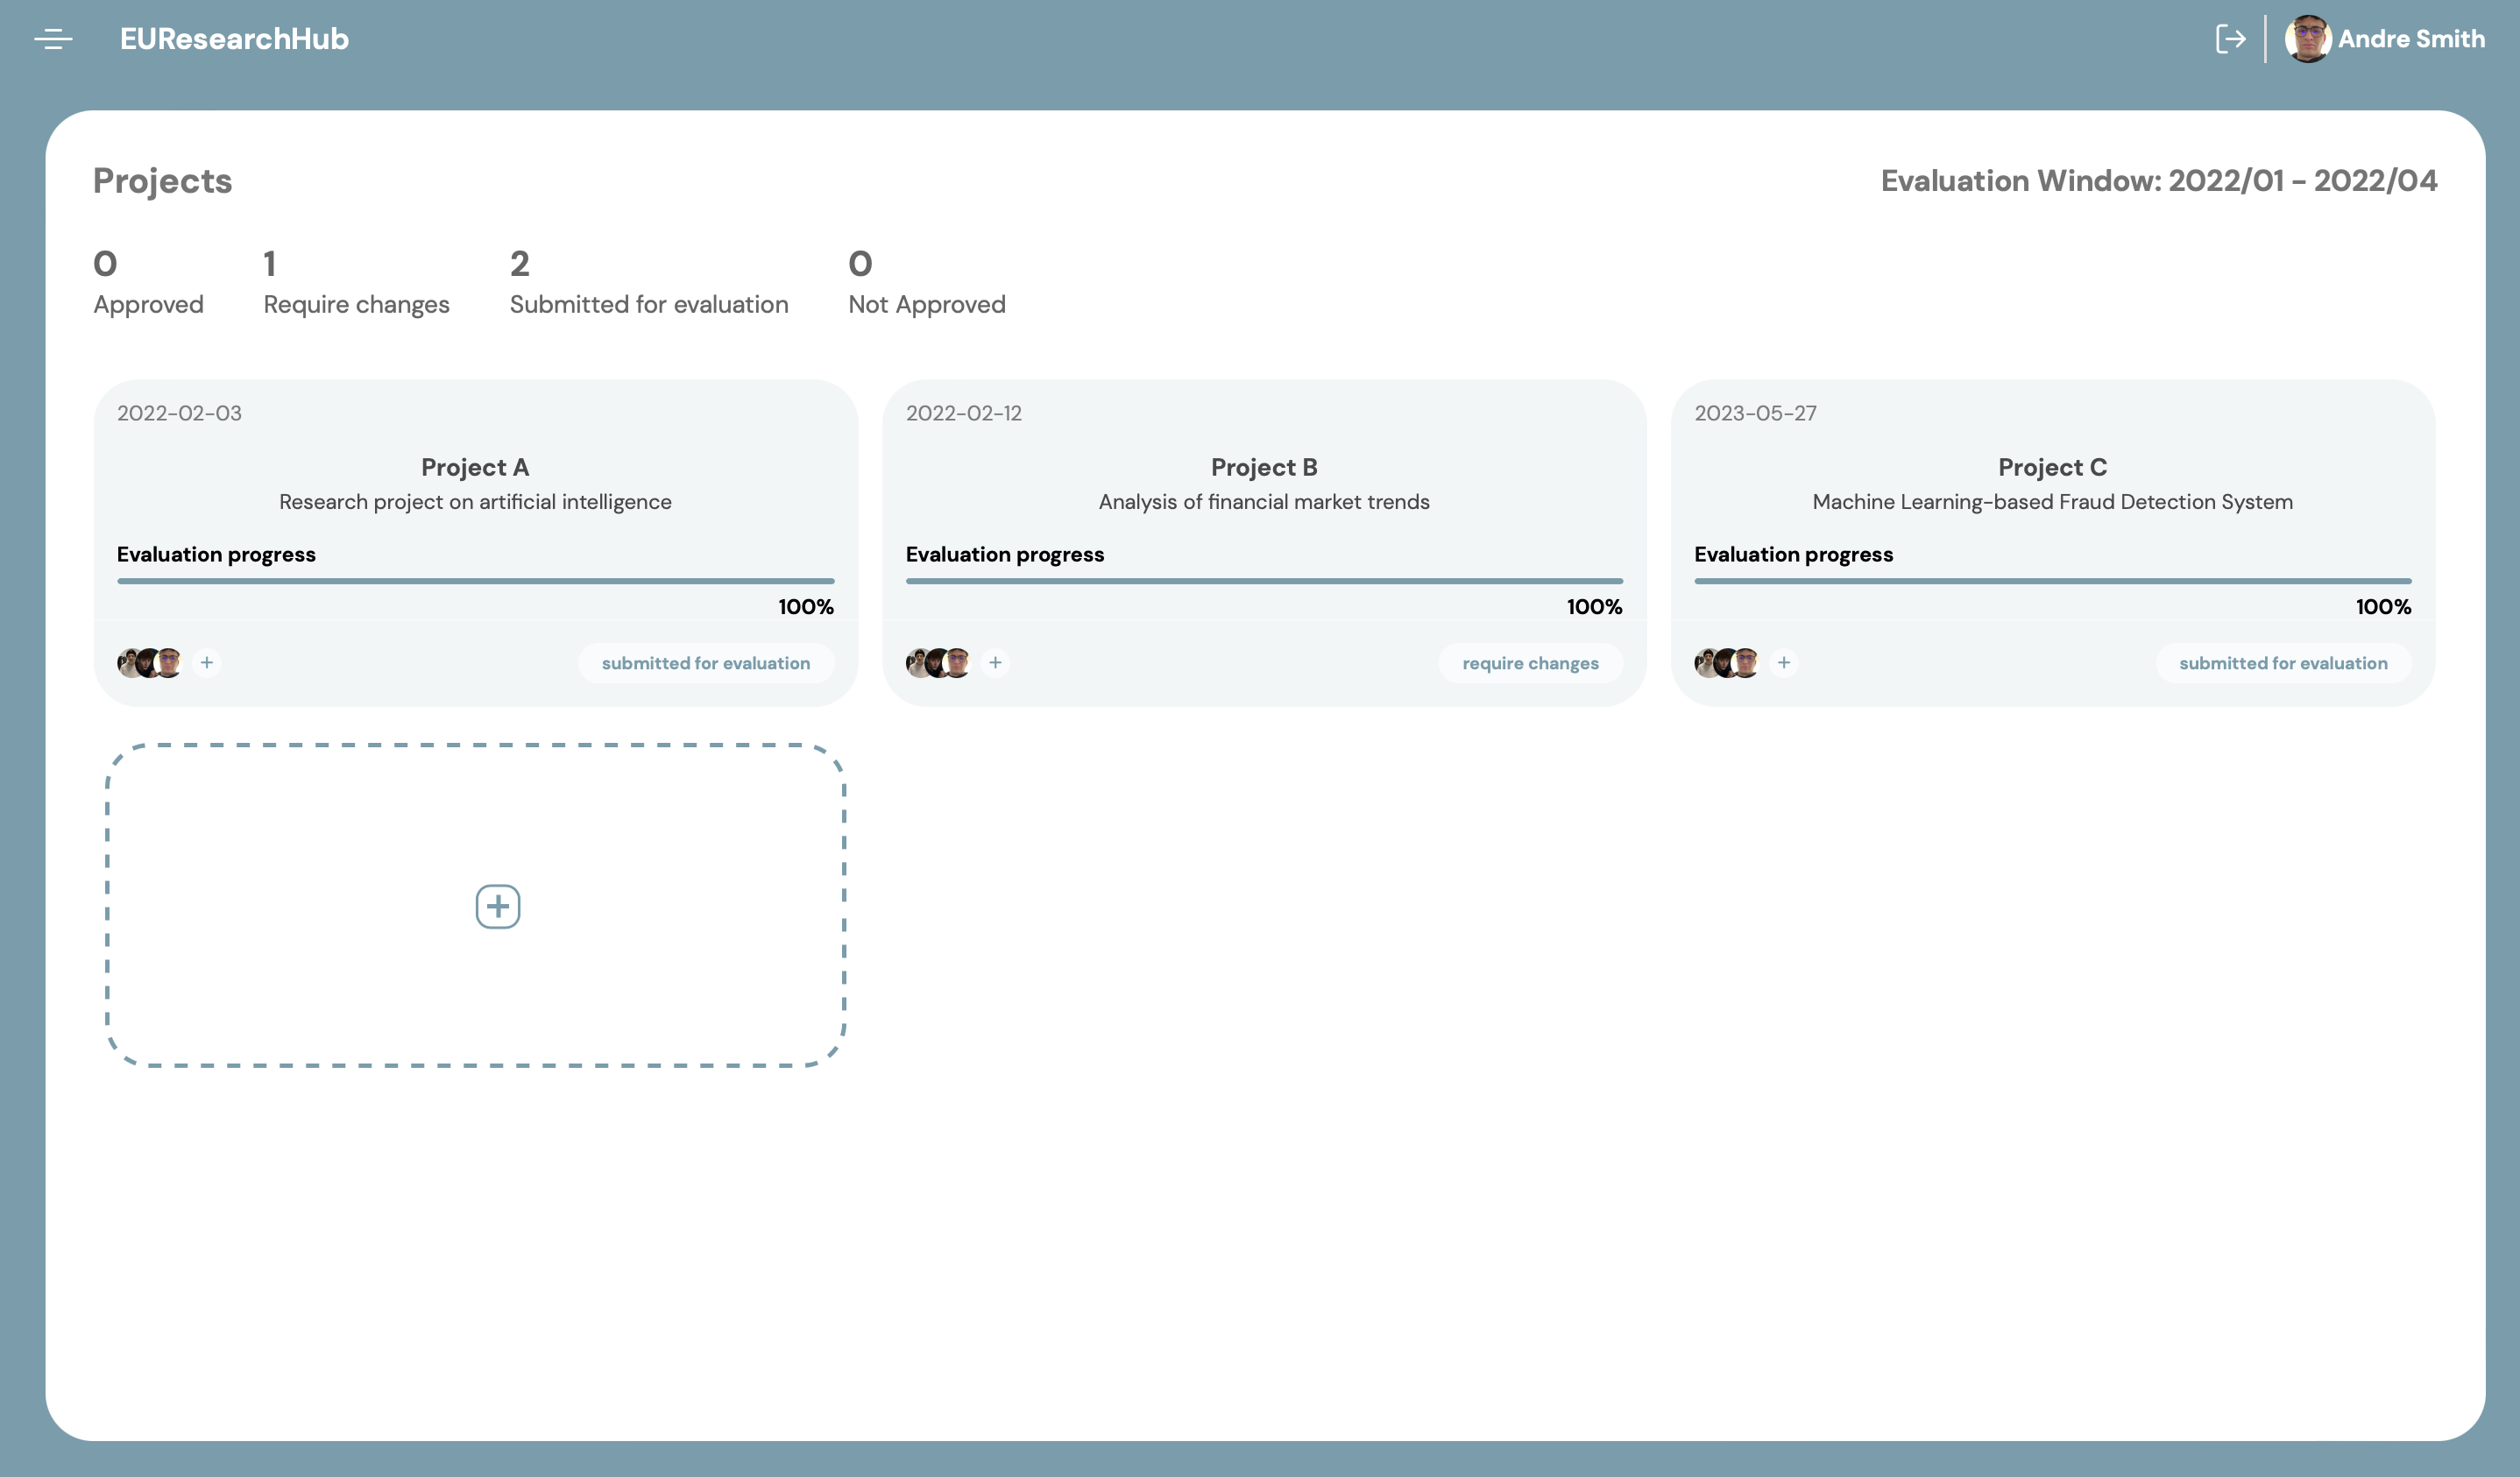
\includegraphics[width=8cm]{10.png} &
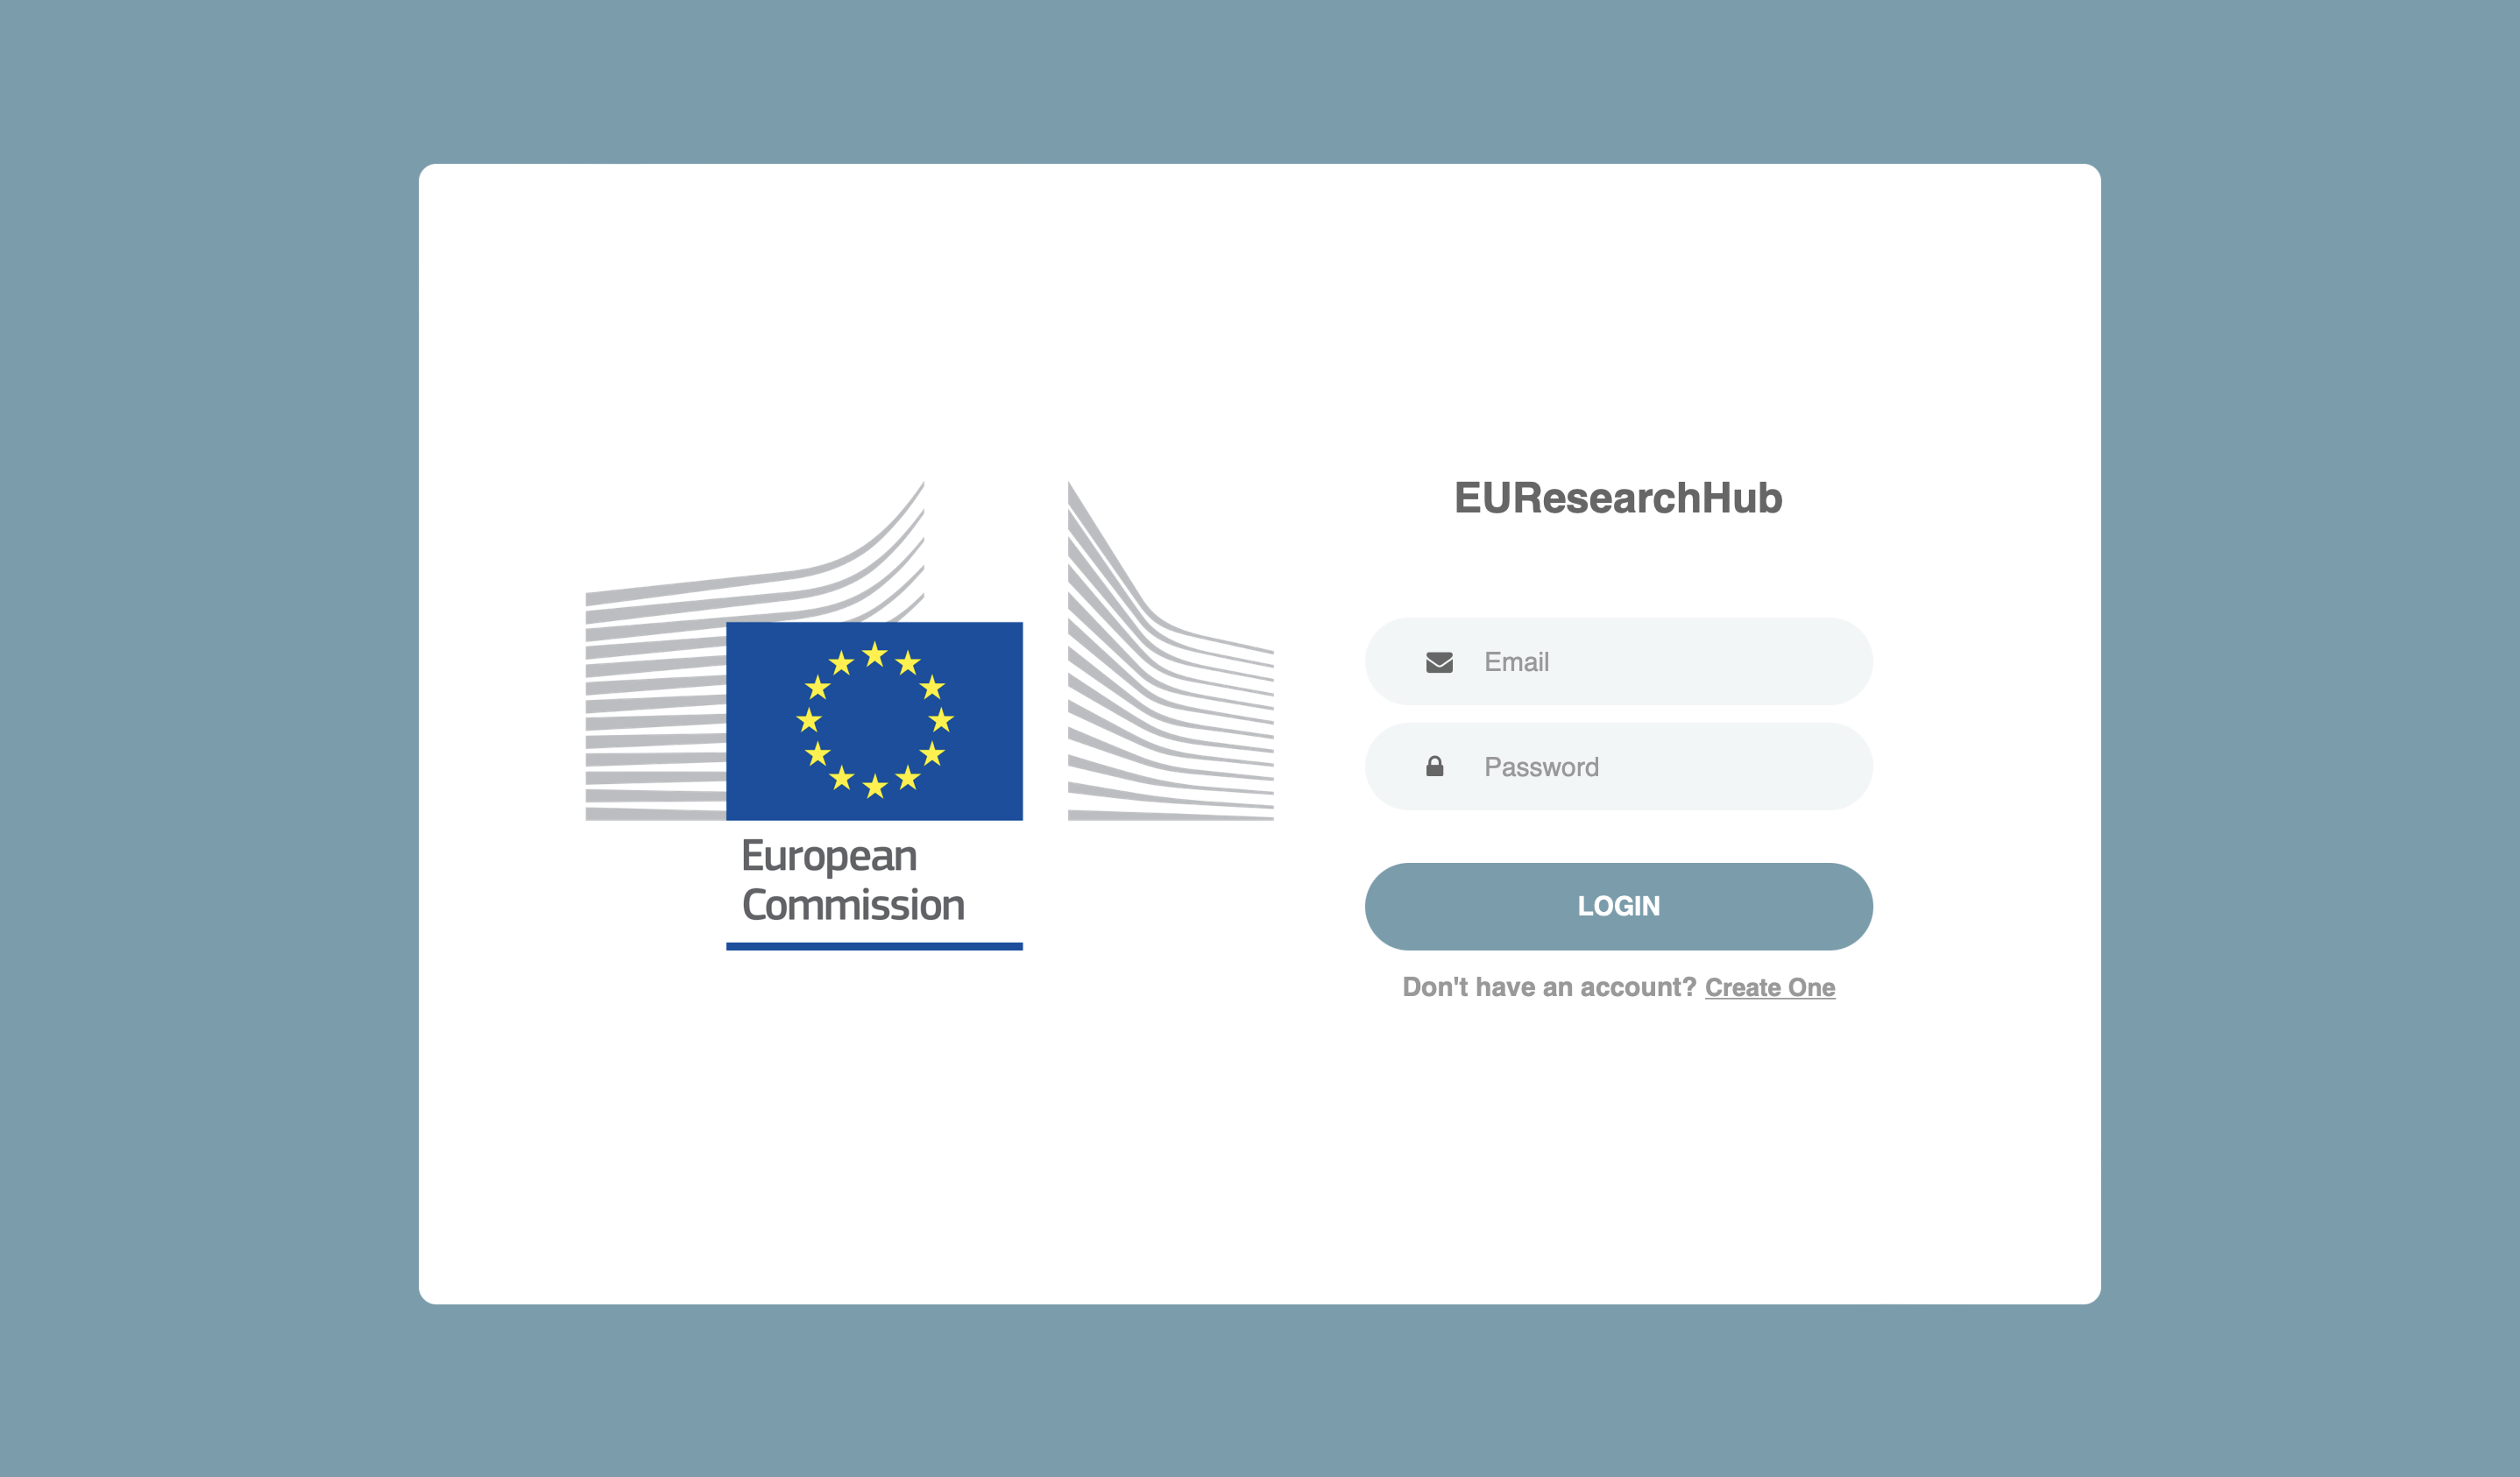
\includegraphics[width=8cm]{11.png} \\
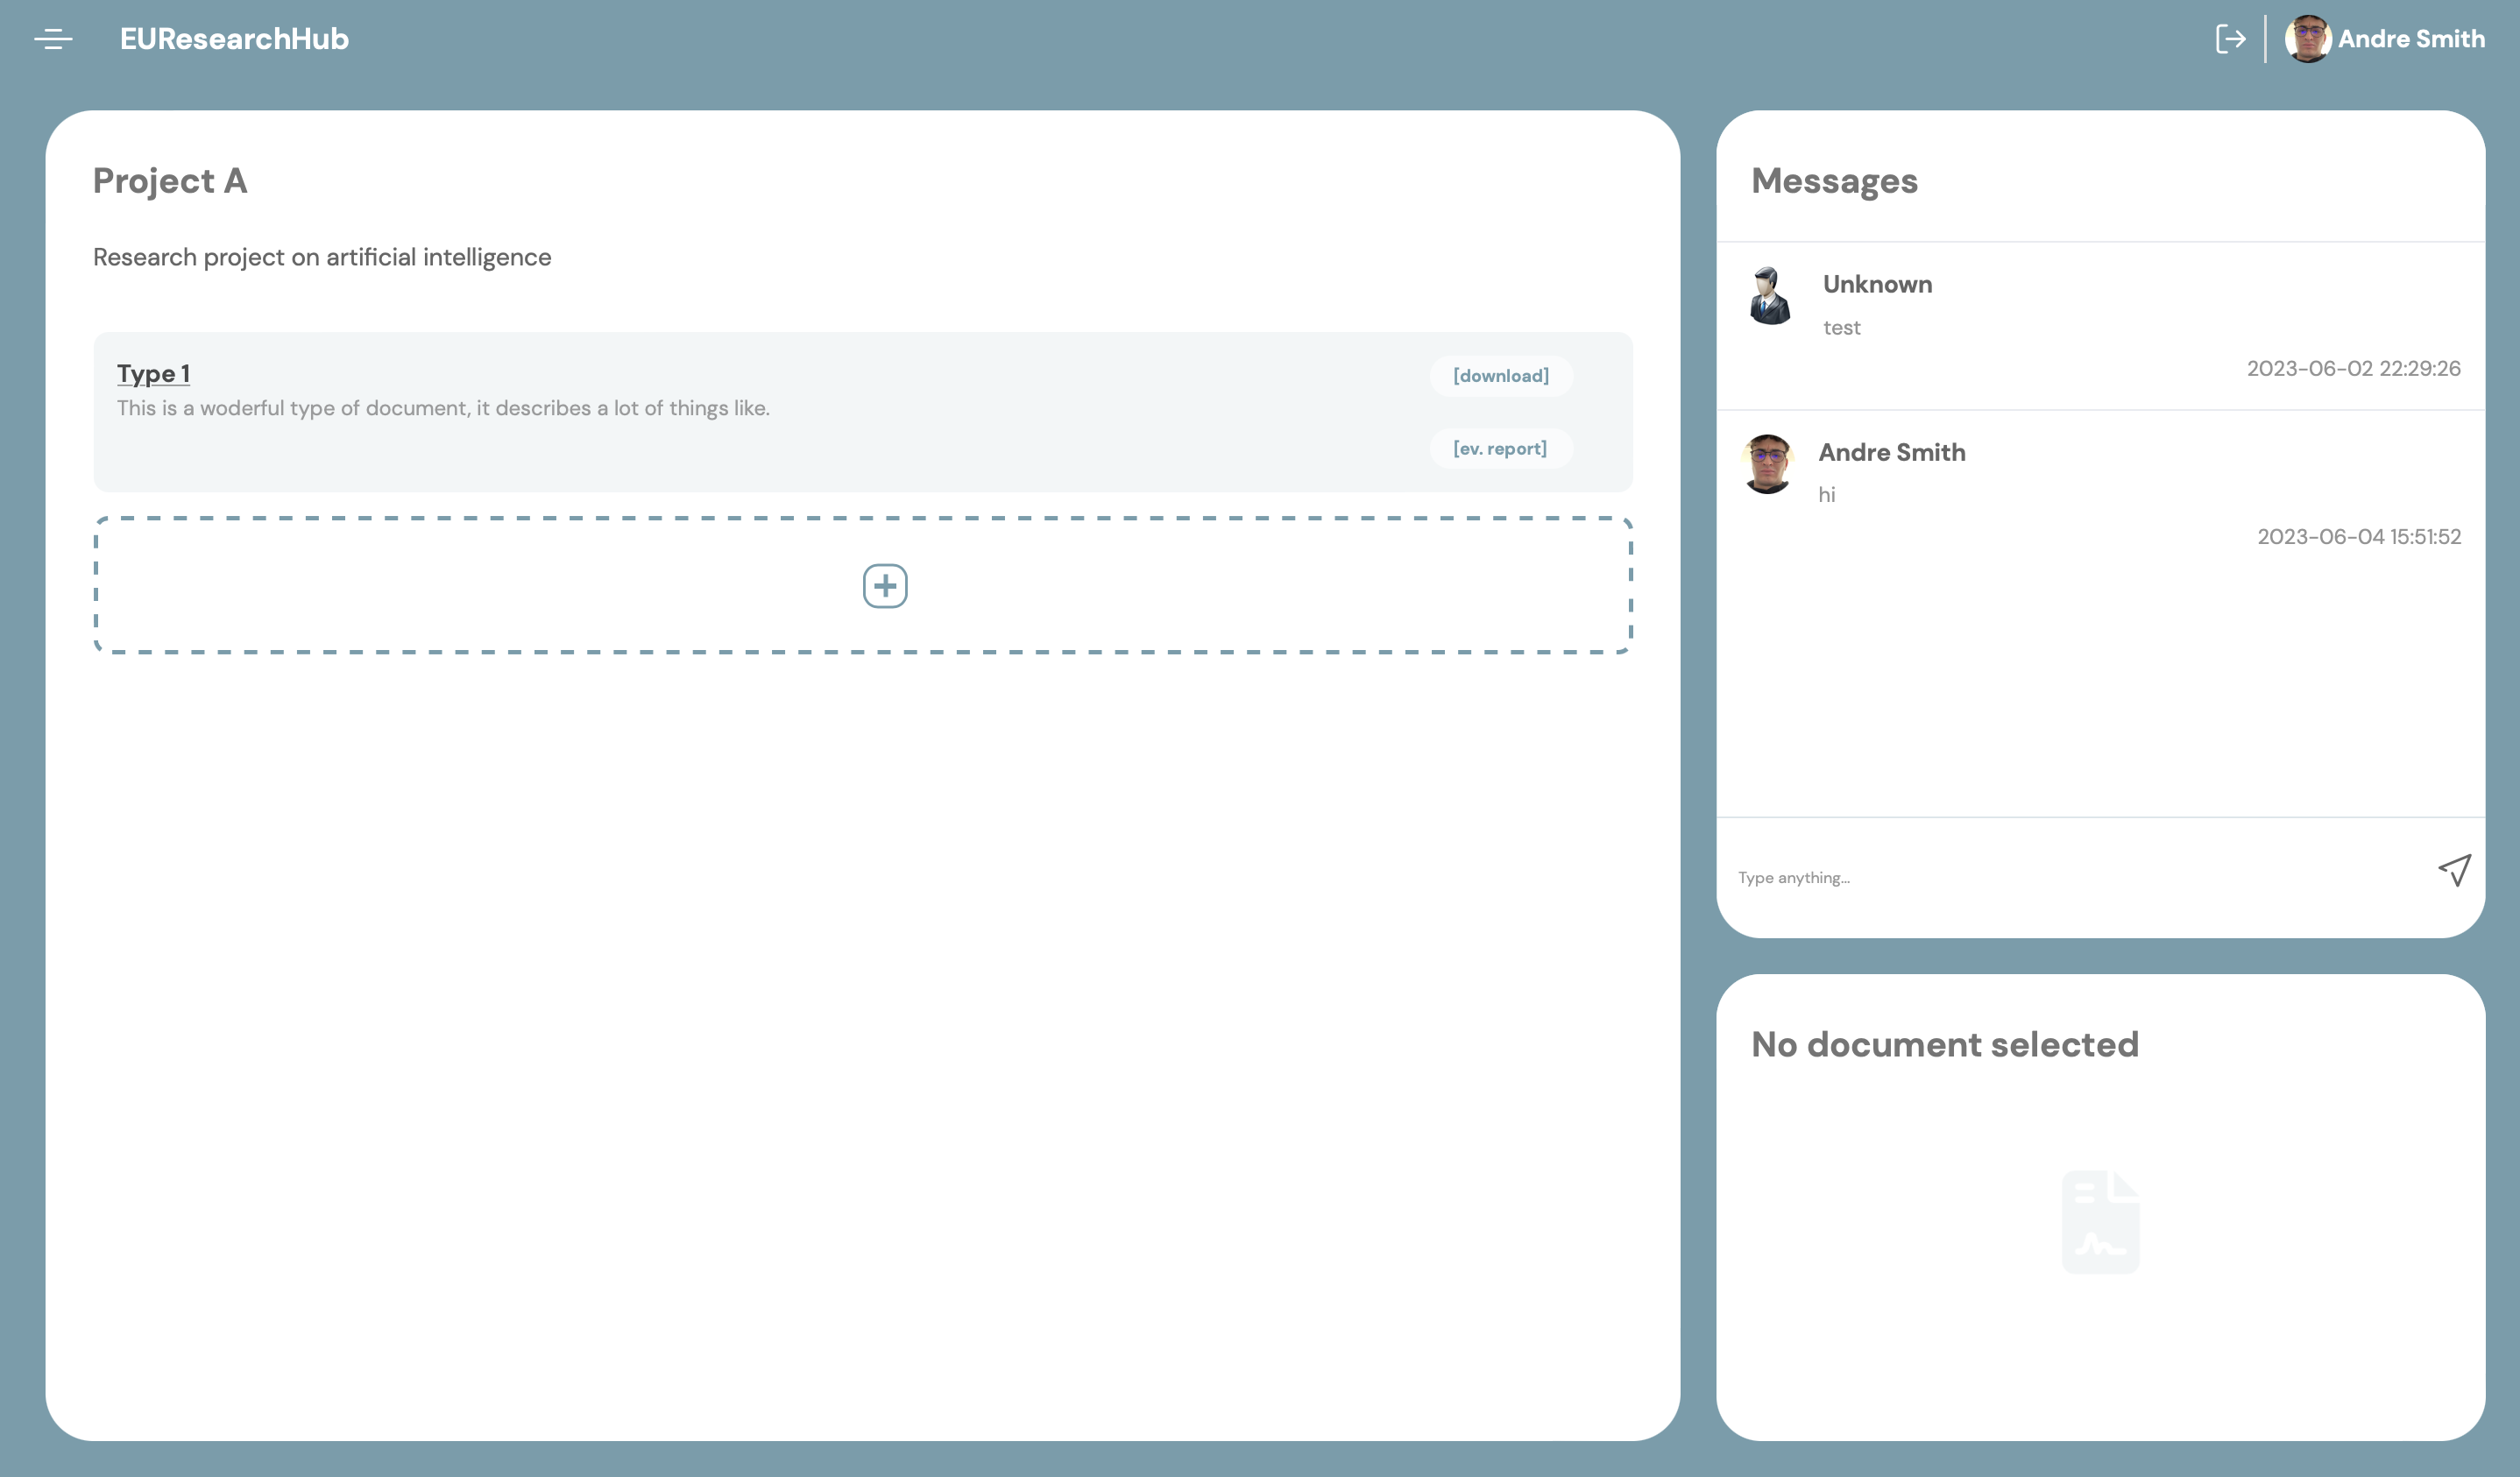
\includegraphics[width=8cm]{12.png} &
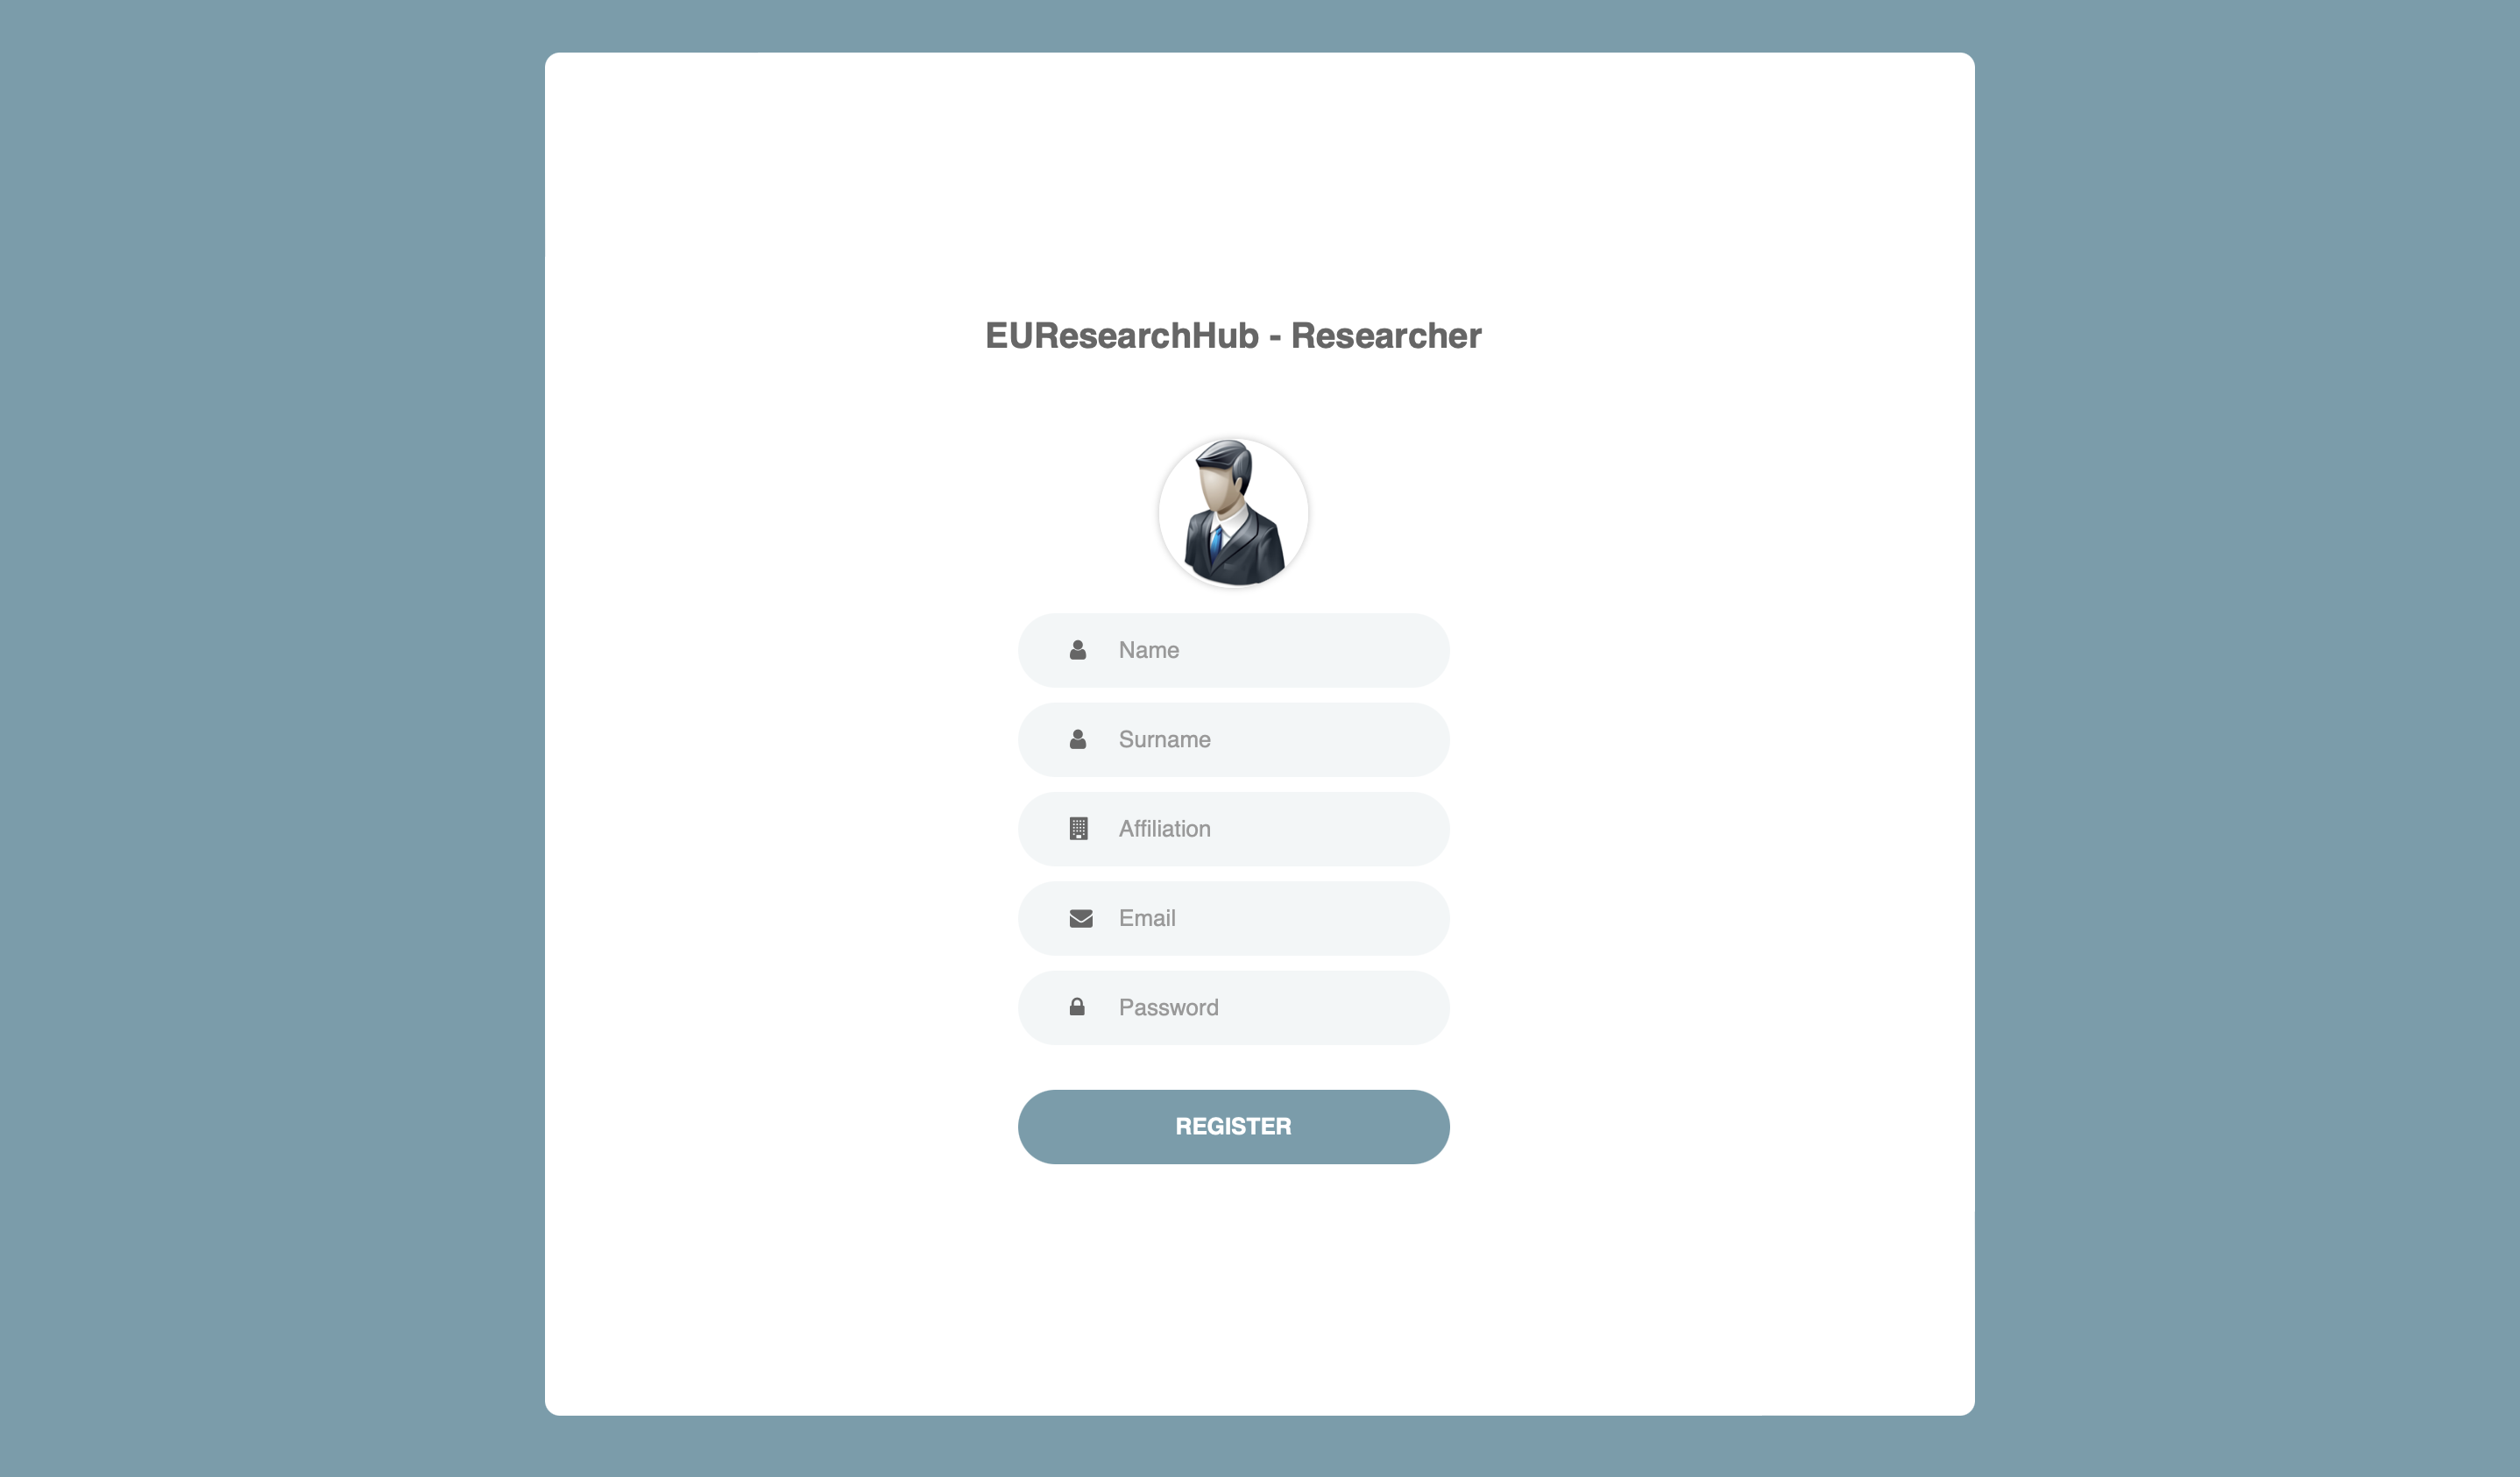
\includegraphics[width=8cm]{13.png} \\
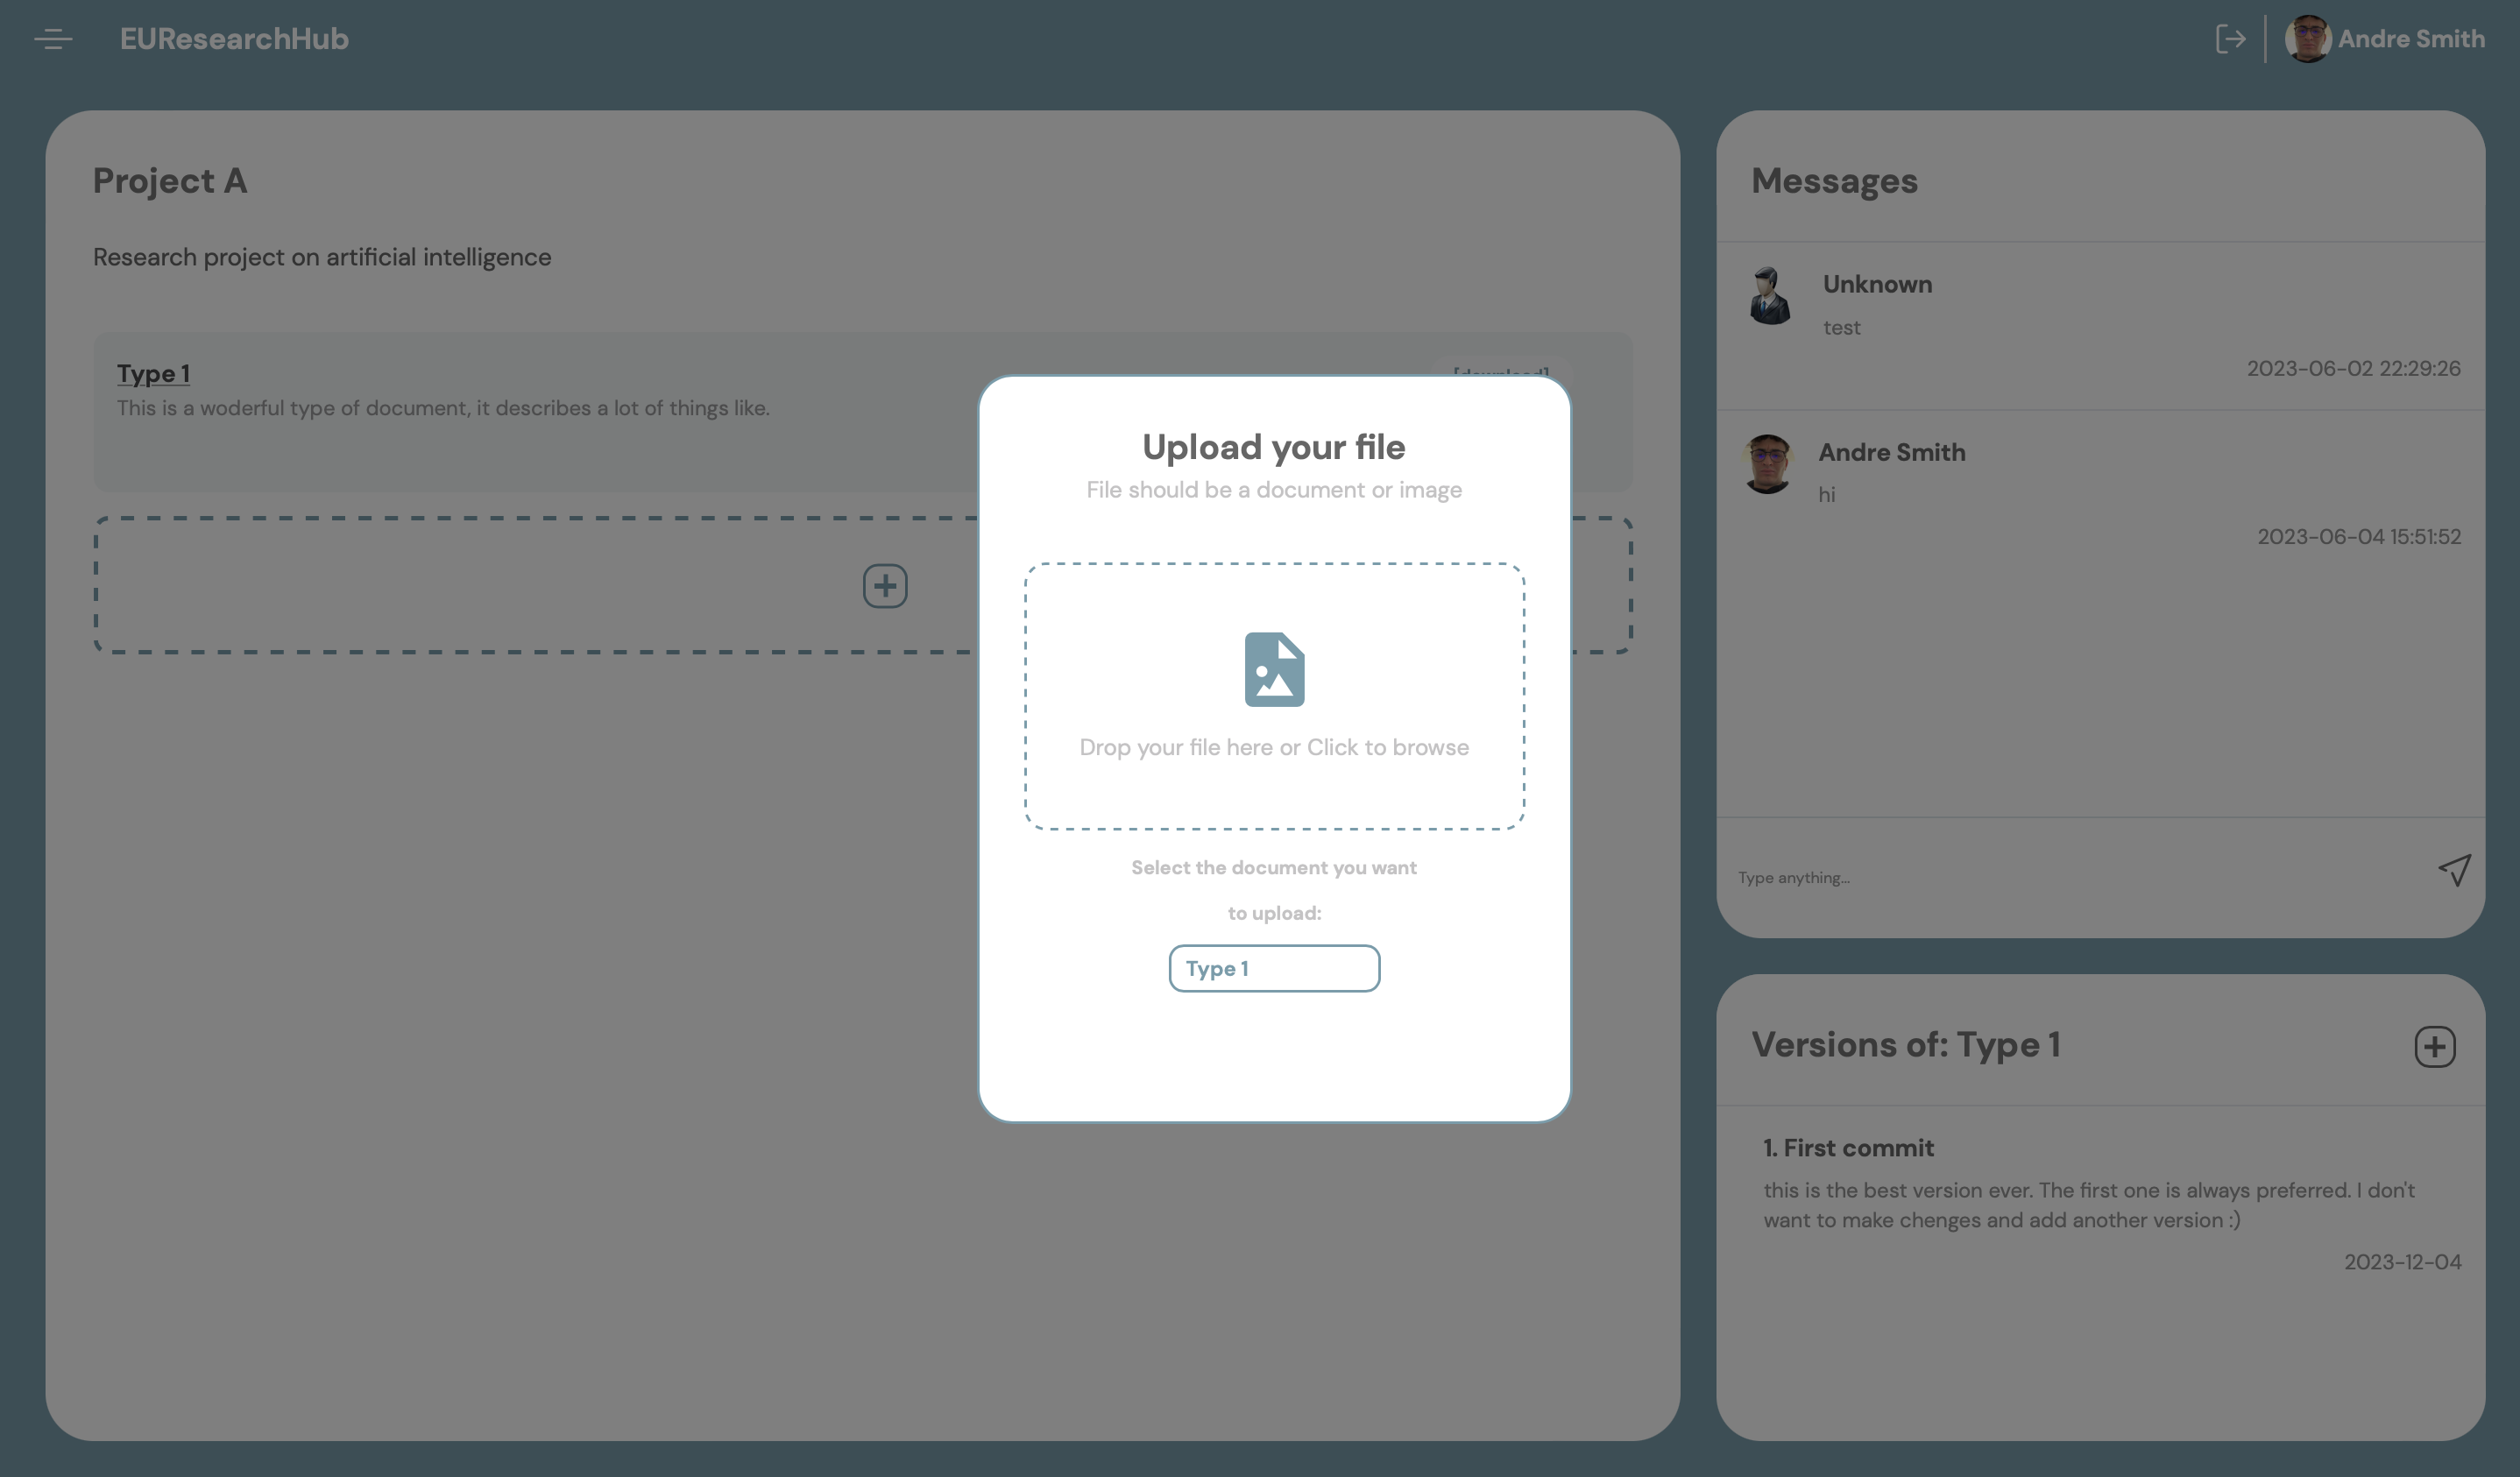
\includegraphics[width=8cm]{14.png} &
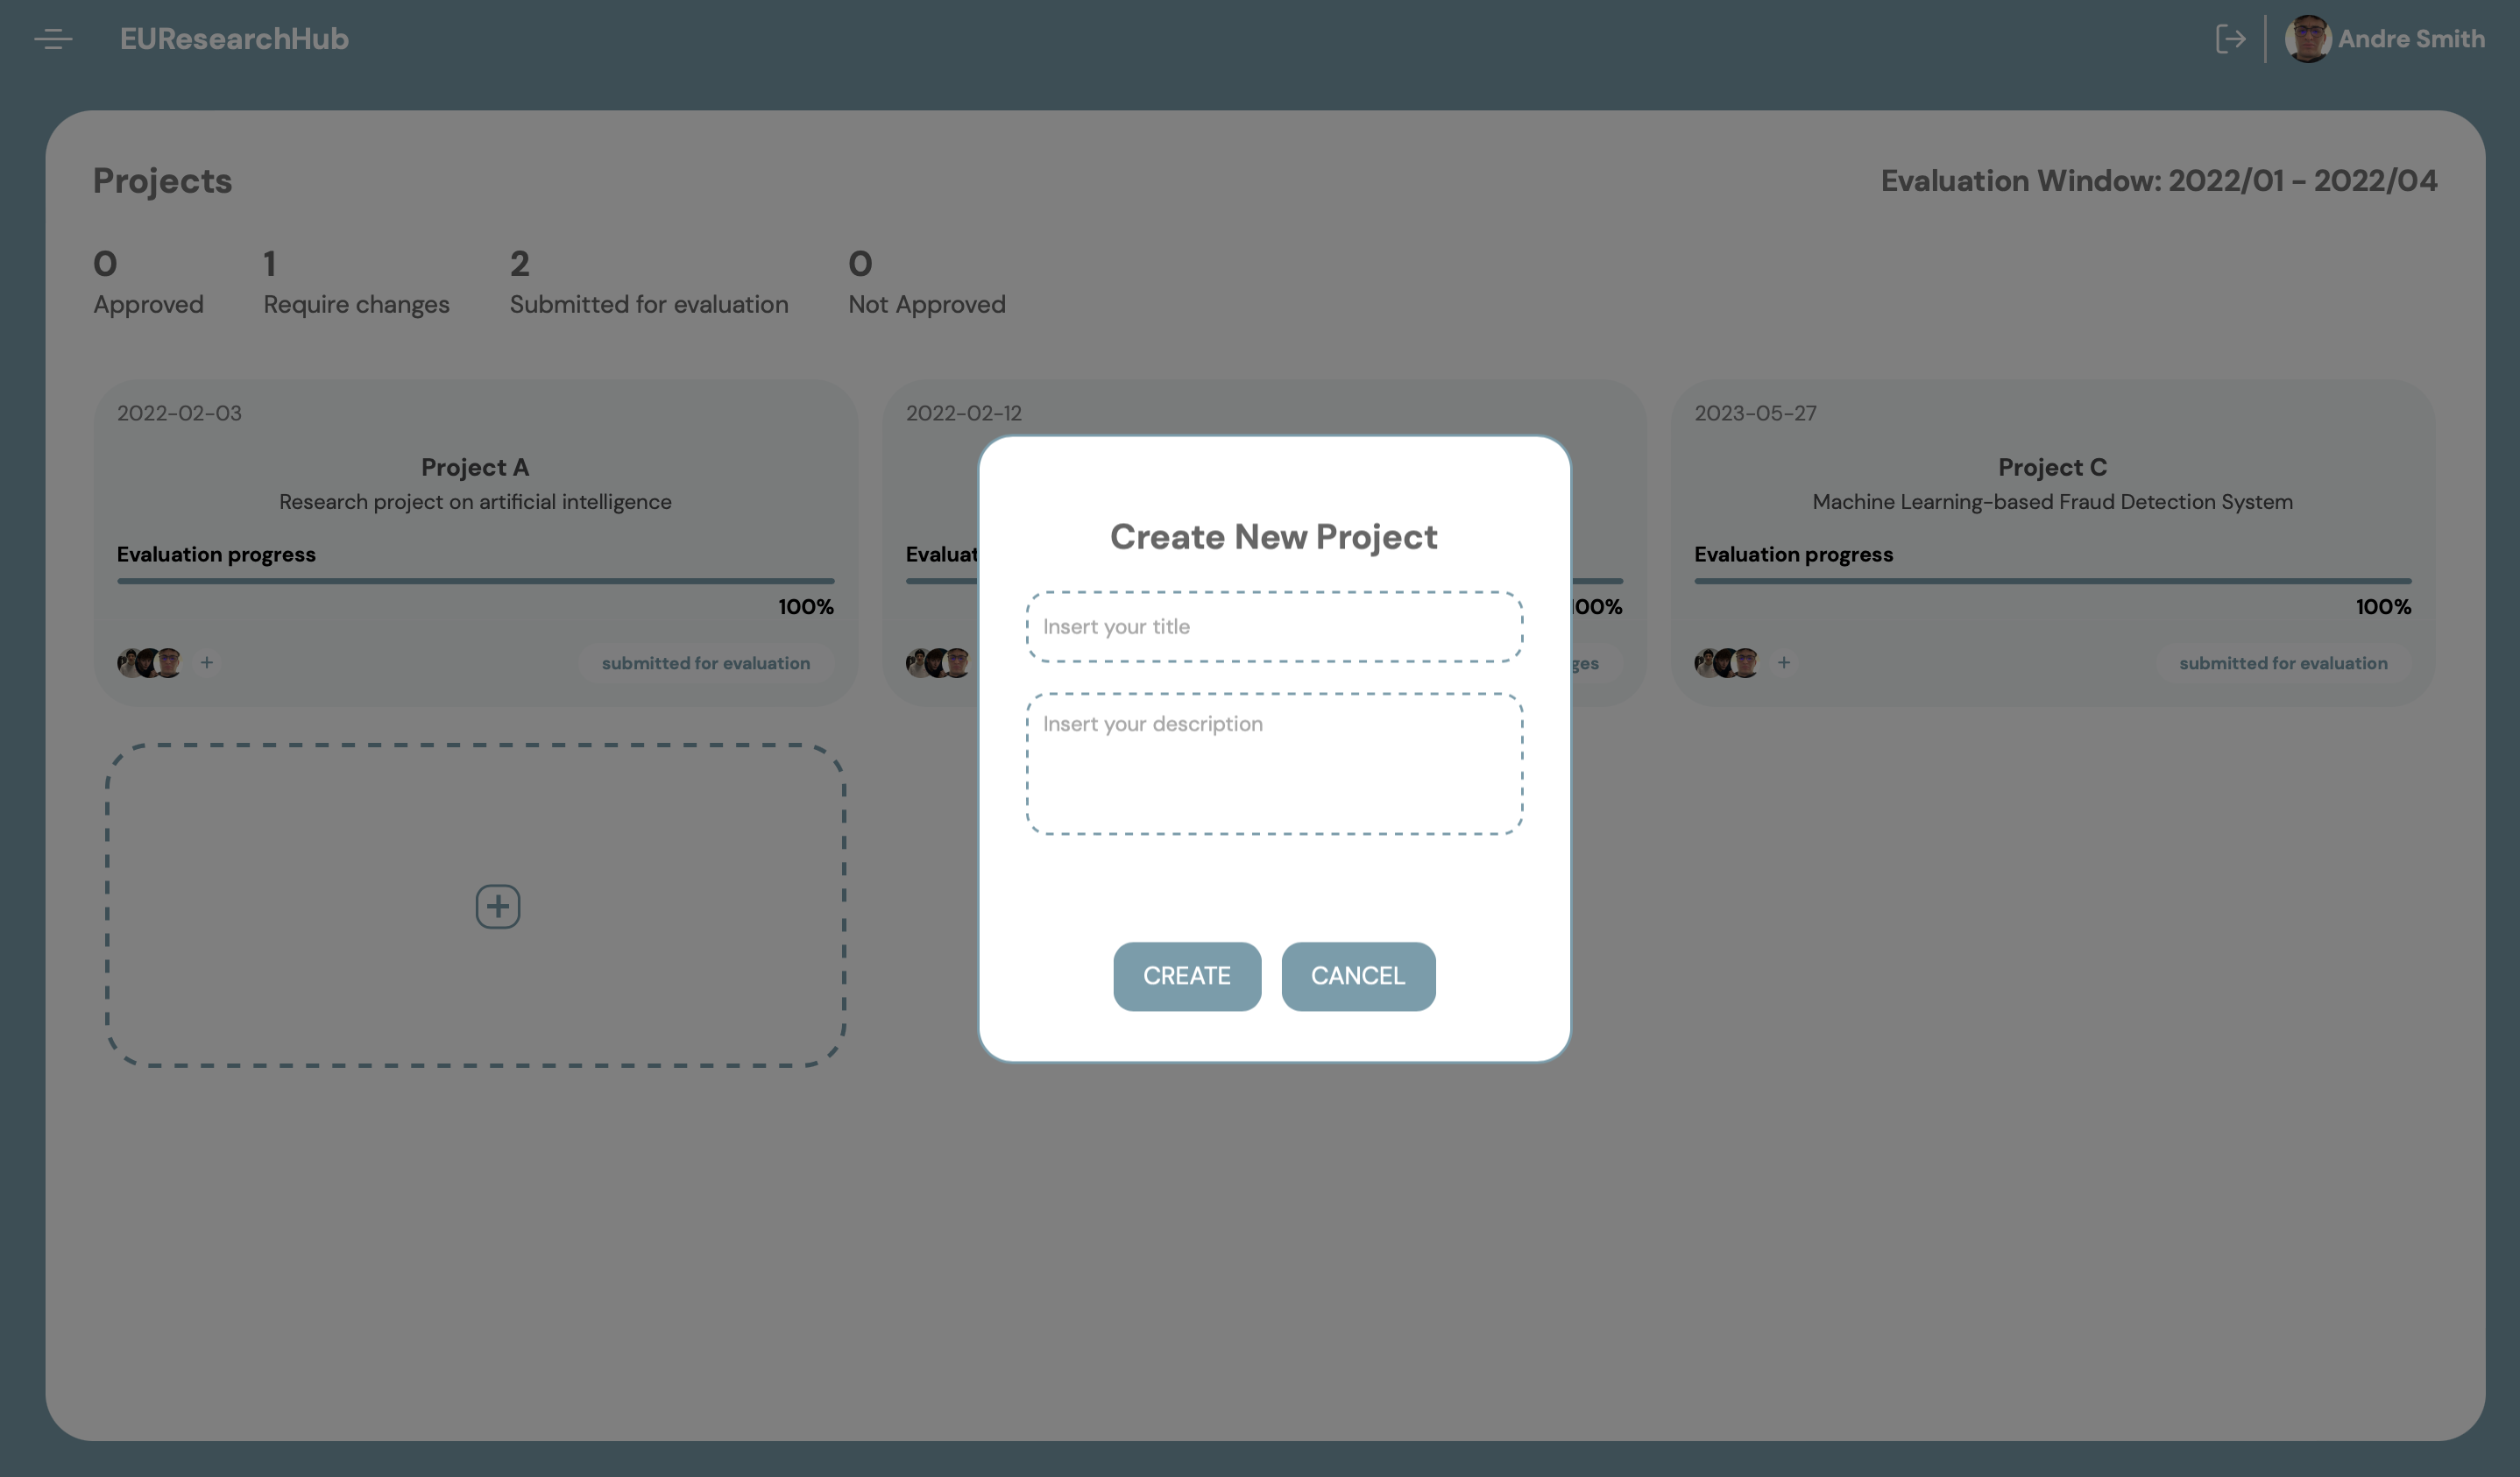
\includegraphics[width=8cm]{15.png} \\
\end{longtable}

\end{center}

\section{Integrazione tra front-end e back-end}

L'integrazione tra il frontend e il backend nel progetto EUResearchHub avviene attraverso richieste HTTP effettuate dal client al server. Il frontend comunica con il backend per inviare e ricevere dati, consentendo all'utente di interagire con l'applicazione e visualizzare i risultati delle operazioni. Le richieste HTTP vengono gestite attraverso un'architettura API (Application Programming Interface), che definisce il modo in cui il frontend e il backend comunicano tra loro. Nel caso di EUResearchHub, vengono utilizzate diverse API per consentire all'utente di eseguire azioni come l'autenticazione, la ricerca di progetti di ricerca e l'invio di messaggi.\\
Durante queste interazioni, possono verificarsi situazioni di errore. Per gestire gli errori, il backend può generare messaggi di errore che vengono restituiti al frontend. Ad esempio, se si verifica un'eccezione durante l'esecuzione di un trigger o se il token di login o CSRF (Cross-Site Request Forgery) non è valido, il backend può generare un messaggio di errore e restituirlo al frontend. \\
Si insericono ora due esempi di richieste AJAX:\\
\begin{minipage}{\linewidth}
\begin{imtaCode}{javascript}
$.ajax({
    url: '/api/get_doc_types',
    type: 'POST',
    datatype: 'json',
    beforeSend: function(xhr) {
        xhr.setRequestHeader('X-CSRF-Token', $('meta[name="csrf-token"]').attr('content'))
    },
    success: (data) => {
        $('#selectDocType').empty() data.forEach(item => {
            $('#selectDocType').append(`<option class="inputdoctype" value="${item.id}">${item.name}</option>`)
        })
    }
})
             \end{imtaCode}
\end{minipage}\\
In questo primo esempio una richiesta AJAX viene utilizzata per ottenere i tipi di documento da visualizzare in un'interfaccia modale. Quando l'utente fa clic su un pulsante per aprire la modale, viene scatenata una funzione che effettua una richiesta AJAX al percorso \imtaInlinecode{latex}{/api/get_doc_types} sul server. Questa richiesta viene inviata tramite il metodo POST e viene specificato che il tipo di dati atteso è JSON. Prima di inviare la richiesta, viene impostato l'header \imtaInlinecode{latex}{X-CSRF-Token} con il valore del token CSRF presente nel meta tag della pagina.
Nel backend, il server riceve la richiesta al percorso \imtaInlinecode{latex}{/api/get_doc_types} e restituisce i tipi di documento come dati JSON. Nel successo della richiesta AJAX, i dati ricevuti vengono utilizzati per popolare una select box nel frontend con gli elementi appropriati.\\
\begin{minipage}{\linewidth}
\begin{imtaCode}{javascript}
var xhr = new XMLHttpRequest();
xhr.open("POST", "/add_participant", true);
xhr.setRequestHeader('Content-Type', 'application/json');
xhr.setRequestHeader("X-CSRFToken", csrfToken); // Include the CSRF token in the request headers
xhr.onreadystatechange = function() {
    if (xhr.readyState === 4) {
        console.log(xhr.responseText);
        window.location.reload(); // Reload the page after the AJAX request completes
    }
};
xhr.send(JSON.stringify({
    projectId: projectId,
    email: email
}));
}
             \end{imtaCode}
\end{minipage}
In questo secondo esempio, invece, la funzione \imtaInlinecode{latex}{addParticipant} viene utilizzata per inviare una richiesta AJAX per aggiungere un partecipante a un progetto. Viene creato un oggetto XMLHttpRequest e viene impostato il metodo, l'URL di destinazione e l'intestazione \imtaInlinecode{latex}{Content-Type} per indicare che i dati inviati sono in formato JSON. Viene inoltre incluso il token CSRF nell'intestazione 'X-CSRFToken'. La risposta alla richiesta viene gestita nella funzione onreadystatechange, che controlla lo stato della richiesta e, se è completata (readyState === 4), esegue un'azione (in questo caso, viene stampata la risposta sulla console e la pagina viene ricaricata con eventuali messaggi di errore (i.e. utente già nel progetto o mail non esistente)).

\chapter{Contributo al progetto}
\section{Processo di sviluppo}

\begin{imtaQuote}
 Il lavoro di squadra divide i compiti e moltiplica il successo.
  \end{imtaQuote}
La divisione del lavoro all'interno del nostro gruppo di progetto per EUResearchHub è stata caratterizzata da un approccio collaborativo e flessibile. Sebbene tutti e tre i membri del gruppo abbiano acquisito competenze in diverse aree, tra cui backend, frontend e progettazione della base di dati, ci siamo impegnati a lavorare insieme su tutti gli aspetti del progetto.\\
Durante il processo di sviluppo, abbiamo adottato la piattaforma di collaborazione GitHub come strumento principale per il controllo delle versioni, la gestione del codice. e anche asseganre task e piannificare il lavoro. Attraverso GitHub, siamo stati in grado di lavorare contemporaneamente sulle diverse componenti del progetto, creare branch separati per le funzionalità in sviluppo e gestire i conflitti durante i merge.\\
Per mantenere un'adeguata comunicazione e allineamento, abbiamo stabilito due sprint settimanali durante i quali ci siamo riuniti in chiamate di allineamento. Durante queste chiamate, abbiamo discusso i progressi fatti, le sfide incontrate e le attività da svolgere nella settimana successiva. Questo ci ha permesso di monitorare l'avanzamento del lavoro, individuare eventuali ritardi o problemi e prendere decisioni condivise per affrontarli.


\section{Analitiche Github}
L'utilizzo di GitHub ci ha anche fornito analitiche e statistiche utili per valutare il contributo individuale e collettivo al progetto. Attraverso le funzionalità di tracciamento di GitHub, abbiamo potuto monitorare il numero di commit effettuati da ciascun membro, le modifiche apportate,  le task e il tipo di task portate a termine, problemi sollevati e risolti, nonché le attività di code review e testing.
In allegato alcune statistiche:


\begin{center}
\begin{longtable}{cc}

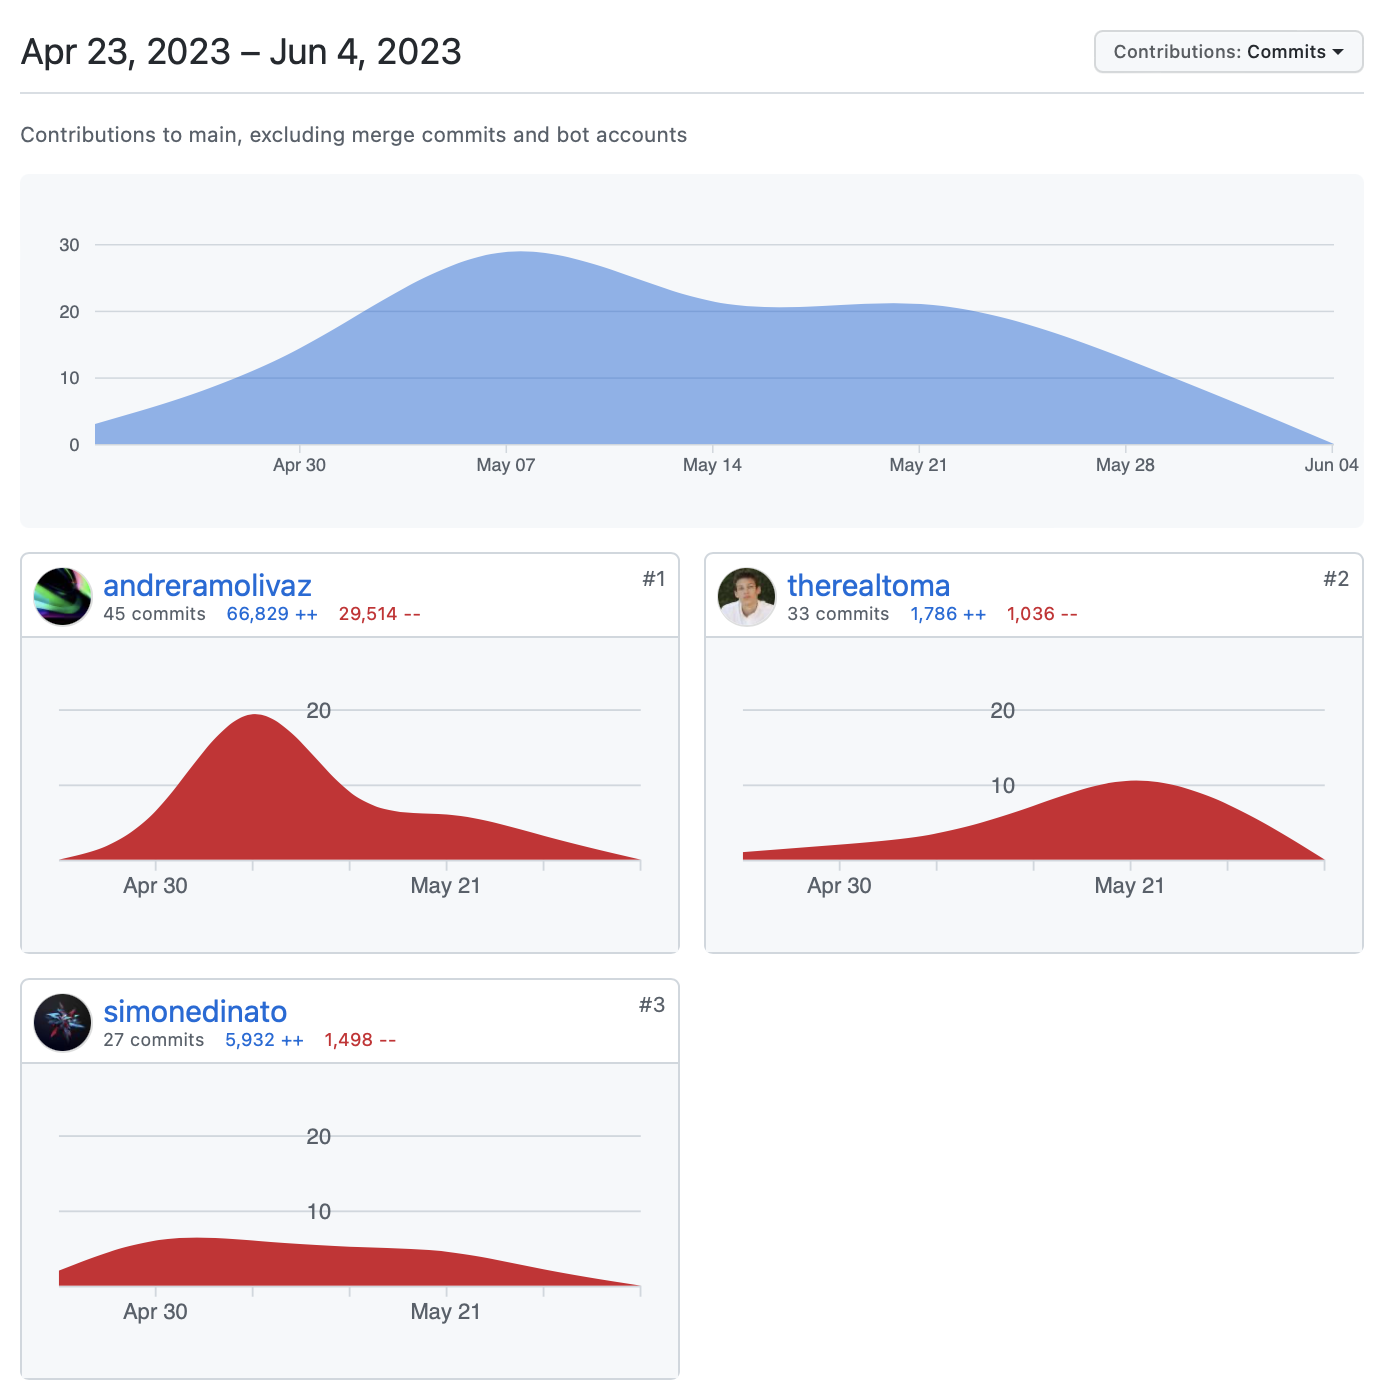
\includegraphics[width=8cm]{16.png} &
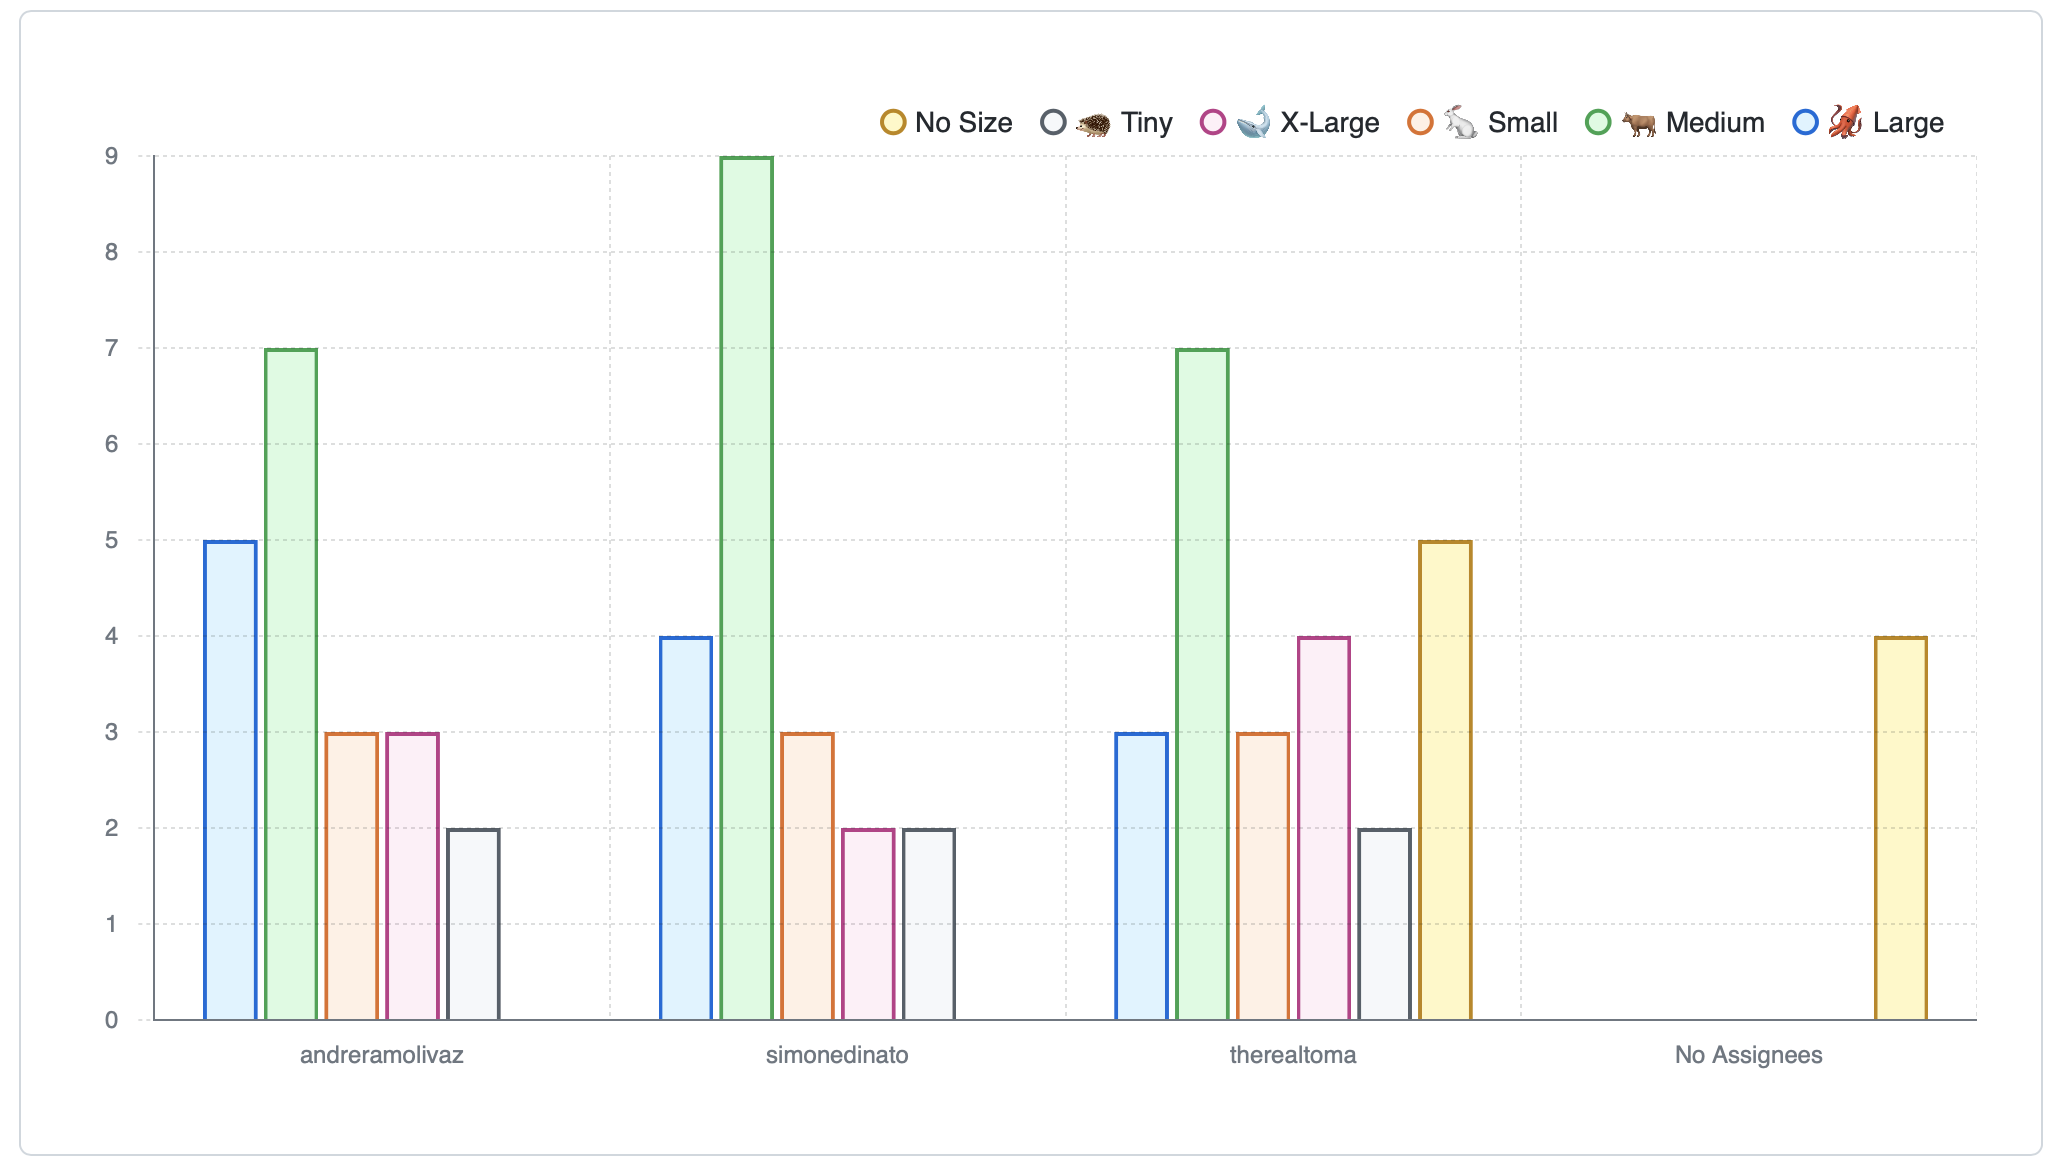
\includegraphics[width=8cm]{17.png} \\

\end{longtable}

\end{center}

\end{document}

%%%%%%%%%% END %%%%%%%%%% 
%%%%%%%%%%%%%%%%%%%%%%%%% 
